% =====================================================================
% CHƯƠNG 5 -- 8
% =====================================================================

\chapter{PHÂN TÍCH VÀ THIẾT KẾ}

\section{Phân tích}

\subsection{Mô hình hóa quy trình nghiệp vụ}
Nghiệp vụ của đề tài được tổ chức thành ba luồng chính chạy song song và hỗ trợ lẫn nhau:

\textbf{Luồng dữ liệu và mô hình (offline):} bắt đầu từ việc thu thập snapshot giao thông định kỳ từ TomTom cho tập đoạn do OpenStreetMap định nghĩa; dữ liệu thô sau đó được làm sạch (khử trùng lặp, xử lý giá trị thiếu), kết hợp đặc trưng hạ tầng và thời tiết, chuẩn hóa, lựa chọn thuộc tính, gom cụm và đánh giá đa chỉ số. Mô hình tốt nhất được xuất ra JSON cho cả ứng dụng di động lẫn server. Hình~\ref{fig:pipeline} mô tả chi tiết quy trình này dưới dạng sơ đồ khối.

\textbf{Luồng người dùng (online, trên ứng dụng):} người dùng đăng nhập, xem bản đồ trạng thái giao thông được tô màu theo cụm, thực hiện tìm đường --- lúc này ứng dụng kết hợp dữ liệu live TomTom, suy luận gom cụm on-device và (khi có) dự báo từ server để chấm điểm và đề xuất tuyến; người dùng có thể phản hồi bằng cách báo sự cố, lưu lịch sử hoặc đánh giá tuyến.

\textbf{Luồng dịch vụ ML (online, server):} ứng dụng gửi đặc trưng của đoạn/tuyến tới server; server chuẩn hóa, suy luận bằng mô hình Random Forest, gán cụm bằng mô hình K-Means dùng chung, tính rủi ro sự cố và trả kết quả; khi không thể kết nối, ứng dụng tự fallback về logic on-device.

\begin{figure}[h!]
\centering
\begin{tikzpicture}[
 font=\small,
 node distance=4mm and 6mm,
 box/.style={draw=brand, fill=brandlight, rounded corners=2pt, minimum height=8mm, minimum width=34mm, align=center, thick},
 data/.style={draw=black!60, fill=white, rounded corners=2pt, minimum height=8mm, minimum width=30mm, align=center},
 arrow/.style={-{Stealth[length=2.5mm]}, thick, black!70}
]
\node[data] (osm) {OpenStreetMap\\(hạ tầng, hình học)};
\node[data, right=of osm] (tomtom) {TomTom Traffic\\(tốc độ, jamFactor)};
\node[data, right=of tomtom] (mapbox) {Mapbox\\(làn xe, matching)};
\node[data, right=of mapbox] (meteo) {Open-Meteo\\(thời tiết ngày)};

\node[box, below=8mm of tomtom, xshift=-18mm] (collect) {Thu thập snapshot\\(171 lần, 09/03--15/04)};
\node[box, right=of collect] (clean) {Làm sạch, khử\\trùng lặp, fill thiếu};
\node[box, below=of clean] (feature) {Chuẩn hóa z-score\\+ lựa chọn thuộc tính\\(MI, RF Importance)};
\node[box, below=of feature] (cluster) {Gom cụm\\(5 thuật toán, $k=2..12$)};
\node[box, right=of cluster] (eval) {Đánh giá đa chỉ số\\(Silhouette, DBI, CH,\\ARI, NMI, FMI)};
\node[box, below=of cluster] (select) {Chọn mô hình tốt nhất\\K-Means $k=6$ (FS)};
\node[box, below=of select, xshift=22mm] (export) {Xuất JSON\\(centroids + scaler)};
\node[box, below=of export] (app) {Nhúng vào\\app Android};
\node[box, left=of app] (server) {Nạp vào\\server ML};
\node[box, right=of app] (rf) {Huấn luyện RF\\dự đoán tốc độ};

\draw[arrow] (osm.south) |- (collect.west);
\draw[arrow] (tomtom.south) -- (collect.north);
\draw[arrow] (mapbox.south) -- (clean.north);
\draw[arrow] (meteo.south) |- (clean.east);
\draw[arrow] (collect) -- (clean);
\draw[arrow] (clean) -- (feature);
\draw[arrow] (feature) -- (cluster);
\draw[arrow] (cluster) -- (eval);
\draw[arrow] (eval.south) |- ($(select.east)+(2mm,0)$) -| (select.east);
\draw[arrow] (select) -- (export);
\draw[arrow] (export) -- (app);
\draw[arrow] (export) -- (server);
\draw[arrow] (export) -- (rf);
\end{tikzpicture}
\caption{Sơ đồ khối quy trình nghiệp vụ của pipeline dữ liệu và học máy.}
\label{fig:pipeline}
\end{figure}

\subsection{Mô hình hóa tương tác}
\subsubsection{Các tác nhân}
Hệ thống có ba tác nhân:
\begin{enumerate}[label=(\roman*),leftmargin=2.2cm,itemsep=2pt]
 \item \textbf{Người dùng} --- người tham gia giao thông sử dụng ứng dụng di động;
 \item \textbf{Quản trị} --- người vận hành pipeline dữ liệu, huấn luyện lại mô hình và giám sát server ML;
 \item \textbf{Hệ thống ngoài} --- các dịch vụ cung cấp dữ liệu và chức năng (TomTom, Google Maps/Routes/Places, Open-Meteo, Firebase, Gemini) tham gia như các tác nhân phụ trợ trong các ca sử dụng.
\end{enumerate}

\subsubsection{Sơ đồ Use Case}
Hình~\ref{fig:usecase} trình bày sơ đồ ca sử dụng tổng thể của hệ thống. Người dùng là tác nhân trung tâm với tám nhóm ca sử dụng chính; Quản trị đảm nhận hai ca sử dụng thuộc phần hậu cần; các hệ thống ngoài tham gia vào hầu hết các ca sử dụng online.

\begin{figure}[h!]
\centering
 \begin{adjustbox}{max width=\textwidth}
\begin{tikzpicture}[
 font=\small,
 uc/.style={draw=brand, fill=brandlight, ellipse, minimum width=42mm, minimum height=9mm, align=center, thick},
 actor/.style={draw=black!70, thick, minimum height=12mm, align=center},
 link/.style={-, black!70, thick}
]
% Hộp hệ thống
\draw[rounded corners=4pt, thick, black!40] (-1.2,-6.4) rectangle (10.6,1.7);
\node[anchor=north east, black!60] at (10.4,1.55) {Hệ thống TraffiGo};

% Tác nhân
\node[actor] (user) at (-3.4,-2.2) {Người dùng\\[1pt]\textit{(người đi đường)}};
\node[actor] (admin) at (-3.4,-5.6) {Quản trị\\[1pt]\textit{(vận hành)}};

% Use cases
\node[uc] (uc1) at (1.9,0.8) {Đăng nhập / xác thực};
\node[uc] (uc2) at (1.9,-0.6) {Xem bản đồ giao thông\\(6 mức theo cụm)};
\node[uc] (uc3) at (6.4,0.8) {Tìm đường, né kẹt,\\đa điểm dừng};
\node[uc] (uc4) at (6.4,-0.6) {Xem dự báo ML\\theo đoạn đường};
\node[uc] (uc5) at (1.9,-2.0) {Đọc tin tức giao thông\\(nghe bài viết)};
\node[uc] (uc6) at (6.4,-2.0) {Tìm địa điểm lân cận,\\gọi xe nhanh};
\node[uc] (uc7) at (1.9,-3.4) {Báo sự cố cộng đồng,\\lưu lịch trình};
\node[uc] (uc8) at (6.4,-3.4) {Trợ lý giọng nói,\\bản đồ ngoại tuyến};
\node[uc] (uc9) at (1.9,-5.2) {Huấn luyện lại\\mô hình};
\node[uc] (uc10) at (6.4,-5.2) {Giám sát server\\(\texttt{/health}, Swagger)};

% Liên kết người dùng
\draw[link] (user) -- (uc1);
\draw[link] (user) -- (uc2);
\draw[link] (user) -- (uc3);
\draw[link] (user) -- (uc4);
\draw[link] (user) -- (uc5);
\draw[link] (user) -- (uc6);
\draw[link] (user) -- (uc7);
\draw[link] (user) -- (uc8);
\draw[link] (admin) -- (uc9);
\draw[link] (admin) -- (uc10);

% Tác nhân hệ thống ngoài
\node[actor, align=center, text width=1.7cm] (ext) at (9.55,-0.3) {Hệ thống ngoài: TomTom, Google, Firebase};
\draw[link, dashed] (uc3) -- (ext);
\draw[link, dashed] (uc4) -- (ext);
\draw[link, dashed] (uc1) -- (ext);
\draw[link, dashed] (uc2) -- (ext);
\end{tikzpicture}%
 \end{adjustbox}
\caption{Sơ đồ Use Case tổng thể của hệ thống.}
\label{fig:usecase}
\end{figure}

\subsubsection{Đặc tả các ca sử dụng chính}
Sáu ca sử dụng quan trọng nhất được đặc tả chi tiết trong các Bảng~\ref{tab:uc1}--\ref{tab:uc5}.

\begin{table}[h!]
\centering
\caption{Đặc tả UC-01: Đăng nhập và xác thực.}
\label{tab:uc1}
\small
\begin{tabularx}{\textwidth}{lX}
\toprule
\textbf{Ca sử dụng} & Đăng nhập và xác thực (UC-01)\\
\midrule
Tác nhân & Người dùng; hệ thống ngoài: Firebase Authentication\\
Tiền điều kiện & Ứng dụng đã cài đặt, có kết nối mạng\\
Luồng chính & \textbf{1.} Người dùng nhập email/mật khẩu hoặc chọn Google Sign-In. \textbf{2.} Firebase Auth xác thực và trả về thông tin người dùng. \textbf{3.} Ứng dụng chuyển tới Trang chủ, tải hồ sơ (tên, avatar Base64) và các địa điểm đã lưu từ Realtime Database.\\
Luồng thay thế & 2a. Sai thông tin đăng nhập: hiển thị thông báo lỗi từ Firebase, giữ nguyên màn hình.\\
 & 2b. Chưa có tài khoản: chuyển sang luồng đăng ký (email/mật khẩu).\\
Kết quả & Phiên đăng nhập được duy trì (tự khôi phục ở lần mở sau); dữ liệu cá nhân sẵn sàng.\\
Yêu cầu liên quan & FR01, FR12, NFR05\\
\bottomrule
\end{tabularx}
\end{table}

\begin{table}[h!]
\centering
\caption{Đặc tả UC-02: Xem bản đồ giao thông.}
\label{tab:uc2}
\small
\begin{tabularx}{\textwidth}{lX}
\toprule
\textbf{Ca sử dụng} & Xem bản đồ giao thông (UC-02)\\
\midrule
Tác nhân & Người dùng\\
Tiền điều kiện & Ứng dụng đã khởi động, người dùng đã đăng nhập\\
Luồng chính & \textbf{1.} Ứng dụng nạp hình học 23.417 đoạn từ \texttt{geometry.csv} trên luồng nền. \textbf{2.} Người dùng di chuyển bản đồ; hệ thống xác định các đoạn trong khung nhìn bằng spatial grid. \textbf{3.} Với mỗi đoạn hiển thị (zoom $\ge$ 14, tối đa 150 đoạn/lần), gọi TomTom Flow lấy tốc độ live. \textbf{4.} Tổng hợp 9 đặc trưng và suy luận gom cụm on-device; tô màu theo thứ hạng nghiêm trọng của cụm; đoạn thiếu dữ liệu tô xám. \textbf{5.} Bấm vào một đoạn: hiện bottom sheet chi tiết kèm thẻ Dự báo ML từ server (nếu khả dụng).\\
Luồng thay thế & 3a. TomTom không có dữ liệu cho đoạn: tô xám, không suy đoán.\\
 & 4a. Chưa nạp xong mô hình: dùng màu mặc định rồi cập nhật khi model sẵn sàng.\\
Kết quả & Bản đồ hiển thị trạng thái giao thông 6 mức màu theo thời gian thực.\\
Yêu cầu liên quan & FR02, FR03, FR04, NFR02, NFR04\\
\bottomrule
\end{tabularx}
\end{table}

\begin{table}[h!]
\centering
\caption{Đặc tả UC-03: Tìm đường và né kẹt.}
\label{tab:uc3}
\small
\begin{tabularx}{\textwidth}{lX}
\toprule
\textbf{Ca sử dụng} & Tìm đường, né kẹt, đa điểm dừng (UC-03)\\
\midrule
Tác nhân & Người dùng; hệ thống ngoài: Google Routes API, TomTom, server ML\\
Tiền điều kiện & Người dùng đã xác nhận điểm đi và điểm đến\\
Luồng chính & \textbf{1.} Ứng dụng gọi Routes API với phương tiện đã chọn (ô tô/xe máy/đi bộ), kèm intermediates nếu có điểm dừng. \textbf{2.} Giải mã polyline, lấy mẫu dọc tuyến và tra dữ liệu live TomTom cho các đoạn ứng viên. \textbf{3.} Chấm điểm tuyến bằng thời gian điều chỉnh theo congestionIndex. \textbf{4.} Gửi các tuyến ứng viên tới \texttt{/api/ml/recommend-route}; nếu server đề xuất tuyến khác, tự chuyển và thông báo. \textbf{5.} Hiển thị thời gian, quãng đường, câu trạng thái, sức khỏe tuyến A--F và ước tính nhiên liệu.\\
Luồng thay thế & 4a. Server offline: giữ nguyên tuyến chọn bằng điểm số on-device, không báo lỗi.\\
 & 1a. Routes API lỗi/quá hạn mức: thông báo nguyên nhân, giữ trạng thái chọn điểm.\\
Kết quả & Tuyến tối ưu được vẽ trên bản đồ kèm thông tin chi tiết; sẵn sàng bắt đầu dẫn đường.\\
Yêu cầu liên quan & FR05, FR06, FR07, FR09, FR10, NFR01, NFR03\\
\bottomrule
\end{tabularx}
\end{table}

\begin{table}[h!]
\centering
\caption{Đặc tả UC-04: Xem dự báo ML theo đoạn đường.}
\label{tab:uc4}
\small
\begin{tabularx}{\textwidth}{lX}
\toprule
\textbf{Ca sử dụng} & Xem dự báo ML theo đoạn đường (UC-04)\\
\midrule
Tác nhân & Người dùng; hệ thống ngoài: server ML, TomTom\\
Tiền điều kiện & Bottom sheet chi tiết đoạn đang mở\\
Luồng chính & \textbf{1.} Ứng dụng tổng hợp đặc trưng của đoạn (tốc độ live, dòng tự do, chiều dài, giới hạn tốc độ, loại đường, giờ, ngày). \textbf{2.} Gọi \texttt{POST /api/ml/predict} với timeout ngắn; lần lượt thử các địa chỉ server mặc định. \textbf{3.} Server chuẩn hóa, suy luận RF trả tốc độ dự đoán, gán cụm K-Means, đánh giá rủi ro sự cố. \textbf{4.} Hiển thị thẻ ``Dự báo ML'': tốc độ $\approx$, mức kẹt, cụm giao thông, rủi ro.\\
Luồng thay thế & 2a. Không kết nối được server nào: thẻ hiển thị ``Server ML không khả dụng'', ứng dụng hoạt động bình thường.\\
Kết quả & Người dùng thấy dự báo ML cho đoạn đang quan sát.\\
Yêu cầu liên quan & FR04, FR08, FR10, NFR01, NFR06\\
\bottomrule
\end{tabularx}
\end{table}

\begin{table}[h!]
\centering
\caption{Đặc tả UC-09: Huấn luyện lại mô hình.}
\label{tab:uc5}
\small
\begin{tabularx}{\textwidth}{lX}
\toprule
\textbf{Ca sử dụng} & Huấn luyện lại mô hình (UC-09)\\
\midrule
Tác nhân & Quản trị\\
Tiền điều kiện & Đã cài môi trường Python và các thư viện theo \texttt{requirements.txt}\\
Luồng chính & \textbf{1.} Cập nhật snapshot mới vào thư mục dữ liệu. \textbf{2.} Chạy \texttt{python train\_model.py}: đọc, làm sạch, join thời tiết, huấn luyện RF, copy mô hình gom cụm, xuất \texttt{speed\_rf.joblib}, \texttt{cluster\_model.json}, \texttt{meta.json} kèm chỉ số đánh giá. \textbf{3.} Khởi chạy lại \texttt{uvicorn app:app}; kiểm tra \texttt{/health} xác nhận mô hình đã nạp kèm số liệu MAE/R$^2$.\\
Luồng thay thế & 2a. Dữ liệu quá ít ($<$ 100 mẫu): dừng và báo lỗi thay vì huấn luyện mô hình kém tin cậy.\\
Kết quả & Mô hình mới sẵn sàng phục vụ; ứng dụng có thể cập nhật \texttt{cluster\_model.json} tương ứng.\\
Yêu cầu liên quan & FR08, NFR06\\
\bottomrule
\end{tabularx}
\end{table}

\subsection{Sơ đồ hoạt động và tuần tự của luồng tìm đường}
Hai sơ đồ dưới đây làm rõ luồng nghiệp vụ phức tạp nhất của hệ thống --- tìm đường kết hợp dự báo ML. Hình~\ref{fig:activity} mô tả luồng hoạt động với hai điểm rẽ nhánh: kiểm tra khả dụng của server ML và quyết định chuyển tuyến; nhánh fallback đảm bảo luồng không bao giờ bị gián đoạn. Hình~\ref{fig:seq} mô tả tương tác tuần tự giữa bốn thực thể với mười thông điệp, từ khi người dùng xác nhận điểm đến tới khi kết quả hiển thị.

\begin{figure}[h!]
\centering
\begin{tikzpicture}[
 font=\small,
 st/.style={draw=brand, fill=brandlight, rounded corners=2pt, minimum height=8mm, text width=68mm, align=center, thick},
 dec/.style={draw=orangec, fill=orangec!8, diamond, aspect=2.6, inner sep=1pt, align=center, thick, font=\scriptsize},
 arrow/.style={-{Stealth[length=2.5mm]}, thick, black!70}
]
\node[st] (s0) at (0,0) {Người dùng xác nhận điểm đi --- điểm đến};
\node[st] (s1) at (0,-1.4) {Gọi Routes API lấy các tuyến ứng viên};
\node[st] (s2) at (0,-2.8) {Giải mã polyline, lấy mẫu dọc tuyến,\\tra dữ liệu live TomTom};
\node[dec] (d1) at (0,-4.7) {Server ML\\truy cập được?};
\node[st] (s3) at (4.2,-6.3) {POST \texttt{/api/ml/recommend-route}\\nhận tuyến đề xuất};
\node[st] (s4) at (-4.2,-6.3) {Chấm điểm on-device theo\\thời gian điều chỉnh~(2.1)};
\node[st] (s5) at (0,-7.9) {Vẽ tuyến: màu theo cụm K-Means,\\tuyến khác tô xám};
\node[st] (s6) at (0,-9.3) {Hiển thị thời gian/quãng đường, sức khỏe\\tuyến A--F, ước tính nhiên liệu};
\node[dec] (d2) at (0,-11.0) {Server chọn tuyến\\khác?};
\node[st, fill=greenc!10] (s7) at (4.2,-12.5) {Chuyển tuyến +\\thông báo cho người dùng};
\node[st, fill=greenc!10] (s8) at (-4.2,-12.5) {Giữ nguyên tuyến\\hiện tại};
\draw[arrow] (s0) -- (s1);
\draw[arrow] (s1) -- (s2);
\draw[arrow] (s2) -- (d1);
\draw[arrow] (d1.east) -| node[above, font=\scriptsize]{Có} (s3.north);
\draw[arrow] (d1.west) -| node[above, font=\scriptsize]{Không} (s4.north);
\draw[arrow] (s3.south) |- (s5.east);
\draw[arrow] (s4.south) |- (s5.west);
\draw[arrow] (s5) -- (s6);
\draw[arrow] (s6) -- (d2);
\draw[arrow] (d2.east) -| node[above, font=\scriptsize]{Có} (s7.north);
\draw[arrow] (d2.west) -| node[above, font=\scriptsize]{Không} (s8.north);
\end{tikzpicture}
\caption{Sơ đồ hoạt động của luồng tìm đường kết hợp dự báo ML.}
\label{fig:activity}
\end{figure}

\begin{figure}[h!]
\centering
\resizebox{0.95\textwidth}{!}{%
\begin{tikzpicture}[
 font=\small,
 life/.style={dashed, black!45, thick},
 msg/.style={-{Stealth[length=2mm]}, thick, black!80},
 ret/.style={-{Stealth[length=2mm]}, thick, black!55, dashed},
 head/.style={draw=brand, fill=brandlight, rounded corners=2pt, minimum height=8mm, align=center, thick, text width=24mm}
]
\node[head] (u) at (0,0) {Người dùng};
\node[head] (a) at (3.6,0) {Ứng dụng TraffiGo};
\node[head] (s) at (7.4,0) {ML Server\\(FastAPI)};
\node[head] (t) at (10.8,0) {TomTom /\\Routes API};
\foreach \x in {0,3.6,7.4,10.8} \draw[life] (\x,-0.5) -- (\x,-9.6);
\draw[msg] (0,-0.8) -- node[above, font=\scriptsize]{1. Chọn điểm đi --- điểm đến} (3.6,-0.8);
\draw[msg] (3.6,-1.5) -- node[above, font=\scriptsize]{2. computeRoutes} (10.8,-1.5);
\draw[ret] (10.8,-2.2) -- node[above, font=\scriptsize]{3. Tuyến + encoded polyline} (3.6,-2.2);
\draw[msg] (3.6,-2.9) -- node[above, font=\scriptsize]{4. Flow live theo từng đoạn} (10.8,-2.9);
\draw[ret] (10.8,-3.6) -- node[above, font=\scriptsize]{5. currentSpeed / freeFlowSpeed} (3.6,-3.6);
\draw[msg] (3.6,-4.3) -- node[above, font=\scriptsize]{6. POST \texttt{/api/ml/recommend-route}} (7.4,-4.3);
\draw[ret] (7.4,-5.0) -- node[above, font=\scriptsize]{7. recommendedId + scores} (3.6,-5.0);
\draw[msg] (3.6,-5.7) -- node[above, font=\scriptsize]{8. POST \texttt{/api/ml/predict}} (7.4,-5.7);
\draw[ret] (7.4,-6.4) -- node[above, font=\scriptsize]{9. predictedSpeed + cụm + rủi ro} (3.6,-6.4);
\draw[ret] (3.6,-7.3) -- node[above, font=\scriptsize]{10. Vẽ tuyến, tô màu cụm, hiển thị dự báo} (0,-7.3);
\node[anchor=west, font=\scriptsize, black!60, text width=118mm] at (0.2,-8.9) {Ngoại lệ: nếu server không phản hồi trong thời gian timeout, các bước 6--9 bị bỏ qua và ứng dụng dùng chấm điểm on-device (nhánh fallback trong Hình~\ref{fig:activity}).};
\end{tikzpicture}%
}
\caption{Sơ đồ tuần tự luồng tìm đường kết hợp dự báo ML.}
\label{fig:seq}
\end{figure}

\section{Giải pháp công nghệ}

\subsection{Front-end (ứng dụng di động)}
Ứng dụng được chọn phát triển \textbf{native trên Android bằng Java} thay vì các framework đa nền tảng. Lý do lựa chọn:
\begin{enumerate}[label=(\roman*),leftmargin=2.2cm,itemsep=2pt]
 \item bản đồ là trung tâm của trải nghiệm --- Google Maps SDK native cho phép can thiệp sâu vào polyline, camera và gesture mà các wrapper đa nền tảng luôn có khoảng cách một lớp;
 \item suy luận gom cụm cần chạy ổn định trên luồng nền với bộ nhớ nhỏ, native Java kiểm soát tốt chi tiết này;
 \item nhóm phát triển đã có sẵn codebase Java ổn định với đầy đủ tính năng, chuyển framework sẽ tạo chi phí rewrite không cần thiết.
\end{enumerate}
Về mặt framework UI, ứng dụng dùng ViewBinding, Material Components (nút pill, chip, bottom sheet) và ViewPager2 cho carousel; đa ngôn ngữ dùng per-app locale của AppCompat.

\subsection{Back-end (server ML)}
\textbf{Lựa chọn: FastAPI + scikit-learn} thay vì hai phương án cân nhắc là Flask và Node.js/Express~\cite{tilkov}. So với Flask, FastAPI có sẵn xác thực schema bằng Pydantic, tự sinh Swagger UI (giảm công sức tài liệu API) và hỗ trợ async. So với kiến trúc Node.js/Express gọi service Python (như đồ án gốc), việc chạy FastAPI \textit{cùng một tiến trình} với mô hình scikit-learn loại bỏ một lớp mạng trung gian, giảm độ trễ và số điểm lỗi, đồng thời vẫn giữ đúng \textit{giao diện API} đã thiết kế trong báo cáo đồ án. Trình tự suy luận trong server: chuẩn hóa đặc trưng $\rightarrow$ Random Forest dự đoán tốc độ $\rightarrow$ K-Means JSON gán cụm $\rightarrow$ luật phát hiện sự cố $\rightarrow$ tổng hợp kết quả trả về.

\section{Thiết kế}

\subsection{Kiến trúc hệ thống}
Hình~\ref{fig:arch} trình bày kiến trúc tổng thể ba tầng của hệ thống.

\begin{figure}[h!]
\centering
 \begin{adjustbox}{max width=\textwidth}
\begin{tikzpicture}[
 font=\footnotesize,
 tier/.style={draw=black!50, rounded corners=4pt, thick, inner sep=4mm},
 comp/.style={draw=brand, fill=brandlight, rounded corners=2pt, minimum height=9mm, text width=32mm, align=center, thick},
 ext/.style={draw=black!60, fill=white, rounded corners=2pt, minimum height=9mm, text width=26mm, align=center},
 arrow/.style={-{Stealth[length=2.5mm]}, thick, black!70},
 bidir/.style={{Stealth[length=2.5mm]}-{Stealth[length=2.5mm]}, thick, black!70}
]
\node[tier, minimum width=148mm, minimum height=27mm] (t1) at (0,0) {};
\node[anchor=west, black!60] at (-7.15,1.72) {\textbf{Tầng ứng dụng (Android)}};
\node[comp] (main) at (-5.25,0.35) {Main\\(hub, carousel)};
\node[comp] (map) at (-1.75,0.35) {TrafficMap\\(bản đồ 6 màu)};
\node[comp] (nav) at (1.75,0.35) {Navigation\\(tìm đường)};
\node[comp] (misc) at (5.25,0.35) {News - Nearby - Profile\\Voice - Ride - History};
\node[comp] (ttc) at (-5.25,-0.95) {\scriptsize \texttt{TomTomTrafficClient}\\(dữ liệu live)};
\node[comp] (cluster) at (-1.75,-0.95) {\scriptsize \texttt{ClusterColorAssigner}\\(K-Means on-device)};
\node[comp] (mlc) at (1.75,-0.95) {\texttt{MlServerClient}\\(OkHttp, fallback)};
\node[comp, text width=28mm] (others) at (5.25,-0.95) {\texttt{FirebaseRTDB}\\(tài khoản, lịch sử)};
\draw[arrow] (map.south) -- (cluster.north);
\draw[arrow] (map.south) -- (mlc.north);
\draw[arrow] (map.south) -- (ttc.north);
\node[tier, minimum width=148mm, minimum height=34mm] (t2) at (0,-4.8) {};
\node[anchor=west, black!60] at (-7.15,-3.02) {\textbf{Tầng dịch vụ (ML Server --- FastAPI)}};
\node[comp] (api) at (-4.7,-4.35) {REST API\\7 endpoint \texttt{/api/ml/*}};
\node[comp] (rfm) at (-1.55,-4.35) {Random Forest\\dự đoán tốc độ};
\node[comp] (kmm) at (1.55,-4.35) {K-Means JSON\\gán cụm};
\node[comp] (inc) at (4.7,-4.35) {Phát hiện\\sự cố};
\node[comp, text width=112mm] (train) at (0,-5.85) {\texttt{train\_model.py}: pipeline huấn luyện\\(scikit-learn + joblib) --- xuất model + meta};
\node[tier, minimum width=148mm, minimum height=20mm] (t3) at (0,-9.2) {};
\node[anchor=west, black!60] at (-7.15,-8.08) {\textbf{Tầng dữ liệu và dịch vụ ngoài}};
\node[ext] (fb) at (-5.25,-8.85) {Firebase Auth\\+ Realtime DB};
\node[ext] (tom) at (-1.75,-8.85) {TomTom\\Flow API};
\node[ext] (goo) at (1.75,-8.85) {Google Maps / Routes / Places};
\node[ext] (wthr) at (5.25,-8.85) {Open-Meteo + CSV snapshot};
\draw[bidir] (mlc.south) -- node[right, font=\scriptsize]{HTTP JSON} (api.north);
\draw[bidir] (ttc.south) -- (tom.north);
\draw[bidir] (others.south) -- (fb.north);
\draw[arrow] (wthr.north) |- (train.east);
\end{tikzpicture} \end{adjustbox}
\caption{Kiến trúc tổng thể ba tầng của hệ thống.}
\label{fig:arch}
\end{figure}

Kiến trúc được tổ chức sao cho \textit{mô hình là tài sản dùng chung}: tệp \texttt{cluster\_model.json} xuất từ pipeline được đặt vào cả \texttt{assets/} của ứng dụng và \texttt{models/} của server, đảm bảo một đoạn luôn được gán về cùng một cụm bất kể nơi suy luận. Tầng ứng dụng giao tiếp với tầng dịch vụ chỉ qua HTTP JSON có timeout ngắn, cho phép hai bên triển khai và cập nhật độc lập.

\subsection{Thiết kế cơ sở dữ liệu}
Dữ liệu người dùng và dữ liệu cộng đồng lưu trên Firebase Realtime Database theo cấu trúc cây JSON Hình~\ref{fig:firebase}; dữ liệu huấn luyện lưu dạng CSV phẳng theo schema 40 cột (Bảng~\ref{tab:schema}).

\begin{figure}[h!]
\centering
 \begin{adjustbox}{max width=\textwidth}
\begin{tikzpicture}[
 font=\small,
 node/.style={draw=brand, fill=brandlight, rounded corners=2pt, minimum height=6.5mm, align=left, thick, font=\small\ttfamily, anchor=west},
 leaf/.style={draw=black!60, fill=white, rounded corners=2pt, minimum height=6mm, align=left, font=\scriptsize\ttfamily, anchor=west},
 arrow/.style={-{Stealth[length=2mm]}, thick, black!70}
]
\node[node] (root) at (0,0) {root};
\node[node] (users) at (1.2,-1.3) {Users/\{uid\}};
\node[node] (inc) at (1.2,-6.7) {incidents/\{id\}};
\node[node] (saved) at (3.6,-2.3) {savedPlaces};
\node[node] (fav) at (3.6,-3.2) {favoritePlaces/\{id\}};
\node[node] (park) at (3.6,-4.1) {parkingSpot};
\node[node] (hist) at (3.6,-5.0) {routeHistory/\{id\}};
\node[node] (avt) at (3.6,-5.9) {avatarBase64};
\node[node] (hw) at (7.0,-2.3) {home $\vert$ work};
\node[leaf] at (9.9,-2.3) {\{address, lat, lng\}};
\node[leaf] at (7.0,-3.2) {\{name, address, lat, lng\}};
\node[leaf] at (7.0,-4.1) {\{address, lat, lng, timestamp\}};
\node[leaf] at (7.0,-5.0) {\{origin/dest, lat, lng, timestamp\}};
\node[leaf] at (7.0,-5.9) {\{chuỗi Base64 (JPEG 256px)\}};
\node[leaf] at (3.6,-7.6) {\{type, lat, lng, timestamp, uid\}};
\draw[arrow] (root.south) |- ($(users.west)+(-2mm,0)$) -- (users.west);
\draw[arrow] (root.south) |- ($(inc.west)+(-2mm,0)$) -- (inc.west);
\draw[arrow] (users.east) -- ($(saved.west)+(-1mm,0)$);
\draw[arrow] (users.east) -- ($(fav.west)+(-1mm,0)$);
\draw[arrow] (users.east) -- ($(park.west)+(-1mm,0)$);
\draw[arrow] (users.east) -- ($(hist.west)+(-1mm,0)$);
\draw[arrow] (users.east) -- ($(avt.west)+(-1mm,0)$);
\draw[arrow] (saved.east) -- (hw.west);
\end{tikzpicture} \end{adjustbox}
\caption{Cấu trúc dữ liệu người dùng trên Firebase Realtime Database.}
\label{fig:firebase}
\end{figure}

Bảng~\ref{tab:fbrules} mô tả chi tiết mục đích từng đường dẫn cùng quy tắc truy cập đề xuất; việc tách quyền theo \texttt{uid} đảm bảo người dùng chỉ đọc/ghi dữ liệu của chính mình, còn nhánh \texttt{incidents} cho phép mọi người dùng đã xác thực cùng báo và đọc sự cố cộng đồng.

\begin{table}[h!]
\centering
\caption{Mô tả đường dẫn dữ liệu và quy tắc truy cập Firebase.}
\label{tab:fbrules}
\small
\begin{tabularx}{\textwidth}{lXX}
\toprule
\textbf{Đường dẫn} & \textbf{Mục đích} & \textbf{Quy tắc truy cập đề xuất}\\
\midrule
\texttt{Users/\{uid\}/savedPlaces/\{home|work\}} & Nhà, công ty phục vụ carousel và phím tắt chỉ đường & Đọc/ghi khi \texttt{auth.uid == \{uid\}}\\
\texttt{Users/\{uid\}/favoritePlaces} & Danh sách địa điểm yêu thích tự đặt tên & Đọc/ghi khi \texttt{auth.uid == \{uid\}}\\
\texttt{Users/\{uid\}/parkingSpot} & Vị trí đỗ xe (đơn, ghi đè mỗi lần lưu) & Đọc/ghi khi \texttt{auth.uid == \{uid\}}\\
\texttt{Users/\{uid\}/routeHistory} & Lịch sử lộ trình, phục vụ ``trải lại tuyến này'' & Đọc/ghi khi \texttt{auth.uid == \{uid\}}\\
\texttt{Users/\{uid\}/avatarBase64} & Ảnh đại diện mã hóa Base64 (JPEG 256px) & Đọc/ghi khi \texttt{auth.uid == \{uid\}}\\
\texttt{incidents/\{id\}} & Sự cố cộng đồng (kẹt, tai nạn, ngập...), tự hết hạn 2 giờ & Đọc/ghi khi \texttt{auth != null}\\
\bottomrule
\end{tabularx}
\end{table}

\begin{table}[h!]
\centering
\caption{Tóm tắt schema tập dữ liệu huấn luyện (40 cột, ví dụ các cột chính).}
\label{tab:schema}
\small
\begin{tabularx}{\textwidth}{>{\raggedright\arraybackslash}p{1.1cm}>{\raggedright\arraybackslash}p{4.4cm}X>{\raggedright\arraybackslash}p{1.7cm}}
\toprule
\textbf{Vị trí} & \textbf{Tên cột} & \textbf{Ý nghĩa} & \textbf{Kiểu}\\
\midrule
0--1 & segmentId, name\_vn & Định danh đoạn (hash), tên đường & text\\
2--5 & lat/lon\_start, lat/lon\_end & Tọa độ hai đầu đoạn & float\\
6--19 & laneCount, speedLimit, ... & Hạ tầng, hình học, độ dốc, cao độ & float/text\\
20--23 & timeStamp, dayOfWeek, hourOfDay, dayType & Ngữ cảnh thời gian (\texttt{yyMMddHHmm}) & int/text\\
24--28 & currentSpeed, freeFlowSpeed, jamFactor, incidentFlag, congestionIndex & Giao thông động (lõi của bài toán) & float\\
29--34 & trafficVolume, LOS, occupancy, crossTime, speedLimitRatio, relativeCongestionIndex & Chỉ số suy diễn phục vụ phân tích & float/text\\
35--39 & route\_distance/duration/weight, congestion\_levels, map\_match\_confidence & Điều hướng và độ tin cậy & float/JSON\\
\bottomrule
\end{tabularx}
\end{table}

\subsection{Thiết kế chi tiết bên trong}

\subsubsection{Suy luận gom cụm on-device (\texttt{ClusterColorAssigner})}
Lớp này đóng gói toàn bộ mô hình gom cụm trên thiết bị. Khi khởi tạo, tệp \texttt{cluster\_model.json} được đọc một lần trên luồng nền. Với mỗi đoạn, 9 đặc trưng được tổng hợp đúng công thức pipeline, chuẩn hóa theo~\eqref{eq:zscore} rồi tìm tâm cụm gần nhất theo khoảng cách Euclid~\eqref{eq:euclid}; thứ hạng nghiêm trọng của cụm được ánh xạ thành 6 màu từ đỏ đậm (kẹt nặng nhất) tới xanh đậm (thoáng nhất). Lớp thành thật dữ liệu (F3): đoạn có \texttt{freeFlowSpeed $\le$ 0} được tô xám ``thiếu dữ liệu'' thay vì suy đoán thành xanh --- tránh tạo ấn tượng sai rằng đường thoáng.

\subsubsection{Định tuyến né kẹt (\texttt{PathFinder})}
Đồ thị được xây dựng với các nút là tọa độ đầu--cuối của đoạn; thuật toán Dijkstra tối ưu theo \textit{thời gian} thay vì khoảng cách, trọng số mỗi cạnh nhân thêm hệ số phạt kẹt:
\begin{equation}
w(s) = \frac{d(s)}{v(s)} \cdot p\!\left(\text{congestionIndex}(s)\right), \qquad p(c) = 1 + 0{,}6 \cdot \frac{0{,}85 - \mathrm{clip}(c,\,0{,}30,\,0{,}85)}{0{,}85 - 0{,}30},
\label{eq:penalty}
\end{equation}
trong đó $d(s)$ là độ dài, $v(s)$ là tốc độ hiện tại của đoạn $s$. Hệ số phạt tối đa 1,6 giúp thuật toán ưu tiên đoạn thoáng mà không dẫn vòng vô lý; giá trị congestionIndex $\le 0$ (không rõ dữ liệu) không bị phạt để tránh bóp méo tuyến.

\subsubsection{Client ML (\texttt{MlServerClient})}
Client OkHttp bất đồng bộ với timeout ngắn (kết nối 1,5s, đọc 4s) nhằm không bao giờ khựng UI; danh sách địa chỉ ứng viên được thử lần lượt (\texttt{10.0.2.2} cho trình giả lập chuẩn, \texttt{127.0.0.1} khi dùng \texttt{adb reverse}, hoặc URL người dùng cấu hình);\footnote{10.0.2.2 là địa chỉ đặc biệt trên trình giả lập Android chính thức, ánh xạ về loopback (127.0.0.1) của máy phát triển; với trình giả lập MuMu/LDPlayer hoặc thiết bị thật, dùng \texttt{adb reverse} hoặc IP LAN.} mọi callback được đưa về UI thread và tự bỏ qua khi activity đã hủy. Cơ chế \textit{generation counter} trong \texttt{NavigationActivity} loại bỏ các callback trả về muộn khi người dùng đã reset giữa chừng --- tránh trạng thái ``tuyến cũ sống lại''.

\subsubsection{Luồng xử lý dữ liệu giao thông trong ứng dụng}
Đây là luồng trung tâm biến dữ liệu thô của TomTom thành trạng thái hiển thị trên bản đồ, tổng hợp trong Hình~\ref{fig:datapipeline}:
\begin{enumerate}[label=\textbf{Bước \arabic*.},leftmargin=2.2cm,itemsep=1pt]
 \item \textbf{Fetch}: với mỗi đoạn trong khung nhìn (zoom $\ge$ 14), \texttt{TomTomTrafficClient} gọi Flow Segment Data API tại hai đầu đoạn và lấy trung bình \texttt{currentSpeed}/\texttt{freeFlowSpeed};
 \item \textbf{Parse}: phản hồi JSON được đọc thành tốc độ hiện tại, tốc độ dòng tự do; lỗi/quota được bắt riêng;
 \item \textbf{Tính chỉ số}: congestionIndex $=$ currentSpeed/freeFlowSpeed, occupancy, relativeCongestionIndex, trafficVolume, crossTime, speedLimitRatio;
 \item \textbf{Phân cụm on-device}: 9 đặc trưng chuẩn hóa bằng scaler rồi tìm tâm cụm gần nhất (\texttt{ClusterColorAssigner});
 \item \textbf{Hiển thị}: thứ hạng nghiêm trọng $\rightarrow$ màu (đỏ đậm $\rightarrow$ xanh đậm); đoạn không có dữ liệu tô xám;
 \item \textbf{Cache + làm mới}: kết quả lưu TTL 3 phút; đoạn ra khỏi khung nhìn được thu hồi.
\end{enumerate}
Cùng một chuỗi xử lý chạy ở phía server cho \texttt{/api/ml/predict} (bước 3-5 thay bằng Random Forest + gán cụm JSON), nhờ đó đặc trưng gửi lên và mô hình suy luận luôn nhất quán.

\begin{figure}[h!]
\centering
\begin{tikzpicture}[
 font=\footnotesize,
 stage/.style={draw=brand, fill=brandlight, rounded corners=2pt, minimum height=9mm, text width=30mm, align=center, thick},
 io/.style={draw=black!60, fill=white, rounded corners=2pt, minimum height=9mm, text width=26mm, align=center},
 arrow/.style={-{Stealth[length=2.5mm]}, thick, black!70}
]
\node[io] (tom) at (0,0) {TomTom Flow API\\(theo đoạn)};
\node[stage] (fetch) at (3.4,0) {1. Fetch\\(zoom $\geq$ 14)};
\node[stage] (parse) at (6.8,0) {2. Parse JSON\\speed/freeFlow};
\node[stage] (feat) at (0,-2.1) {3. Tính 9 đặc trưng\\(congestionIndex...)};
\node[stage] (km) at (3.4,-2.1) {4. K-Means on-device\\(nearest centroid)};
\node[stage] (render) at (6.8,-2.1) {5. Tô màu 6 mức\\(theo thứ hạng)};
\node[stage] (cache) at (3.4,-4.0) {6. Cache TTL 3 phút\\+ thu hồi khỏi view};
\node[io] (mlsrv) at (6.8,-4.0) {ML Server\\(thẻ dự báo)};
\draw[arrow] (tom) -- (fetch);
\draw[arrow] (fetch) -- (parse);
\draw[arrow] (parse.south) |- ($(feat.east)+(2mm,0)$) -- (feat.east);
\draw[arrow] (feat) -- (km);
\draw[arrow] (km) -- (render);
\draw[arrow] (render.south) |- ($(cache.east)+(1mm,0)$) -- (cache.west);
\draw[arrow, dashed] (km.south) -- (mlsrv.north);
\end{tikzpicture}
\caption{Luồng xử lý dữ liệu giao thông trong ứng dụng (fetch $\rightarrow$ xử lý $\rightarrow$ gom cụm $\rightarrow$ hiển thị).}
\label{fig:datapipeline}
\end{figure}

\subsubsection{Tối ưu bản đồ (\texttt{TrafficMapActivity})}
Nạp hình học 23.417 đoạn chạy trên luồng nền và công bố kết quả qua các biến \texttt{volatile} (tránh đọc thấy trạng thái dở dang); chỉ mục không gian dạng lưới ô $\approx$ 900m giúp tra đoạn theo khung nhìn trong $O(1)$ thay vì quét tuyến tính; dữ liệu live có TTL 3 phút; gọi TomTom chỉ khi zoom $\ge$ 14 và tối đa 150 đoạn/lần render, ưu tiên gần tâm màn hình --- cân bằng giữa độ tươi dữ liệu và quota API.

\subsubsection{Tin tức giao thông (\texttt{TrafficNewsActivity})}
Tin tức tổng hợp từ năm báo điện tử (VnExpress, Thanh Niên, Tuổi Trẻ, Dân Trí, VietNamNet) $\times$ năm danh mục, tất cả 25 URL RSS đều được xác minh thật. Ba điểm thiết kế đáng chú ý:
\begin{enumerate}[label=(\roman*),leftmargin=2.2cm,itemsep=2pt]
 \item kết quả từ các nguồn về không đồng bộ nên danh sách được \textit{sắp xếp lại theo thời gian phát} mỗi khi một nguồn phản hồi, tránh bài báo bị ``bó cụm'' theo thứ tự nguồn;
 \item phân tích ngày phát phải thử ba định dạng khác nhau vì các báo không thống nhất (RFC822 năm 4 chữ số, RFC822 năm 2 chữ số, kiểu Mỹ M/d/yyyy);
 \item ảnh đại diện bài viết lấy từ hai vị trí khác nhau tùy nguồn (thẻ \texttt{<img>} trong mô tả hoặc thẻ \texttt{<enclosure>}).
\end{enumerate}
Chức năng ``nghe bài'' scrape nội dung qua WebView với bộ chọn CSS riêng cho từng báo và ba lớp fallback, có timeout tự phục hồi 6 giây.

\subsubsection{Trợ lý giọng nói (\texttt{VoiceAssistantActivity})}
Trợ lý dùng Gemini với cơ chế \textit{function calling bắt buộc} (\texttt{tool\_config.mode = ANY}): giọng nói chuyển thành văn bản, Gemini trả về một \texttt{VoiceIntent\{action, args\}} có cấu trúc, ứng dụng điều phối tới đúng tính năng (dẫn đường, xem kẹt xe, đọc tin, gọi xe, chia sẻ vị trí, mở bản đồ ngoại tuyến...).\footnote{Khóa Gemini trên gói miễn phí giới hạn khoảng 20 yêu cầu/ngày cho mô hình flash; khi vượt hạn mức, lỗi \texttt{RESOURCE\_EXHAUSTED} được bắt và hiển thị thông báo rõ cho người dùng thay vì im lặng.} Nút micro được gắn toàn cục qua \texttt{ActivityLifecycleCallbacks} --- bất kỳ màn hình nào có view id \texttt{btnVoiceMic} đều tự có trợ lý mà không cần lặp code. Giọng phản hồi dùng TTS tiếng Việt; thất bại khởi tạo TTS (thường gặp trên trình giả lập) được ghi nhận và hiển thị thông báo thay vì im lặng.

\subsection{Thiết kế giao diện}
Giao diện được thiết kế theo một hệ định danh trực quan thống nhất áp dụng cho mọi màn hình:
\begin{enumerate}[label=(\roman*),leftmargin=2.2cm,itemsep=2pt]
 \item màu chủ đạo tím thương hiệu \texttt{\#5C4FE0} cho nút hành động chính, chip được chọn và các điểm nhấn;
 \item nền sáng, thẻ bo góc lớn 16--28dp, nút dạng pill;
 \item header trắng với icon tối và tiêu đề in đậm;
 \item chip outline khi chưa chọn, fill tím khi chọn;
 \item bảng màu trạng thái giao thông cố định sáu mức (đỏ đậm $\rightarrow$ xanh đậm).
\end{enumerate}
Bộ thiết kế này đồng bộ toàn bộ 20 màn hình của ứng dụng, giúp trải nghiệm liền mạch như một sản phẩm duy nhất. Một số màn hình tiêu biểu được minh họa trong mục kết quả ứng dụng (mục~\ref{sec:appresults}, Chương 6).

\section{Kết chương}
Chương này đã phân tích ba luồng nghiệp vụ, mô hình hóa tương tác bằng sơ đồ use case kèm sáu đặc tả chi tiết cùng sơ đồ hoạt động và sơ đồ tuần tự cho luồng phức tạp nhất, lựa chọn công nghệ front-end/back-end kèm so sánh phương án, và thiết kế hệ thống ở bốn mức: kiến trúc ba tầng, cơ sở dữ liệu, chi tiết bên trong và giao diện. Các thiết kế này là bản vẽ thi công cho chương hiện thực kế tiếp.

% =====================================================================
\chapter{HIỆN THỰC VÀ KIỂM THỬ}

\section{Hiện thực}

\subsection{Pipeline dữ liệu}
Bộ công cụ thu thập được viết bằng Python, gọi TomTom Flow API theo tọa độ hai đầu từng đoạn trong khung giờ định sẵn và lưu snapshot theo tên tệp \texttt{traffic\_hcm\_<ngày>\_<giờ>.csv}. Trong giai đoạn 09/03--15/04/2026, hệ thống thu được \textbf{171 snapshot} (khoảng 170.000 dòng, 917 đoạn duy nhất). Pipeline làm sạch: loại dòng thiếu cột lõi, chuẩn hóa kiểu dữ liệu, giới hạn miền giá trị hợp lý (tốc độ trong $(0;150)$ km/h, giờ trong $[0;23]$, ngày trong $[0;6]$) và khử trùng lặp theo \texttt{segmentId}; kết quả còn \textbf{149.023 mẫu}. Dữ liệu thời tiết ngày cho TP.HCM (38 ngày) được lấy từ Open-Meteo Archive và join theo ngày được suy ra từ \texttt{timeStamp}, phủ \textbf{100\% mẫu}. Bảng~\ref{tab:dist} thống kê phân bố của tập dữ liệu theo ngữ cảnh thời gian; có thể thấy giờ cao điểm chiếm gần một phần ba số mẫu và có congestionIndex trung bình thấp hơn (kẹt hơn theo quy ước của đề tài) so với ngoài giờ cao điểm --- tín hiệu hợp lý cho thấy dữ liệu phản ánh đúng nhịp sinh hoạt giao thông.

\begin{table}[h!]
\centering
\caption{Phân bố tập dữ liệu theo ngữ cảnh thời gian ($n = 169.897$ mẫu).}
\label{tab:dist}
\small
\begin{tabular}{lrrr}
\toprule
\textbf{Nhóm} & \textbf{Số mẫu} & \textbf{Tỉ lệ} & \textbf{congestionIndex TB}\\
\midrule
Giờ cao điểm (7--9h, 17--19h) & 54.670 & 32{,}2\% & 0{,}751\\
Ngoài giờ cao điểm & 115.227 & 67{,}8\% & 0{,}809\\
Ngày thường & 125.167 & 73{,}7\% & 0{,}781\\
Cuối tuần & 44.730 & 26{,}3\% & 0{,}818\\
\bottomrule
\end{tabular}
\end{table}

Thời gian chạy toàn bộ nhánh Feature Selection (từ đọc dữ liệu tới sinh hình ảnh phân tích) khoảng 70 giây trên máy cá nhân.

\subsection{Kết quả lựa chọn thuộc tính và gom cụm}
Nhãn trạng thái giao thông tham chiếu phục vụ đánh giá ngoại bộ được xây dựng từ tốc độ tương đối và ngưỡng LOS. Hai phương pháp lựa chọn thuộc tính (Mutual Information và Random Forest Importance) được chạy song song; đánh giá top-$k$ cho thấy tập 10 thuộc tính là cân bằng tốt nhất giữa thông tin giữ được và số chiều. Nhánh Feature Selection (10 thuộc tính) sau đó được so sánh với nhánh tìm tham số giữ nguyên 40 thuộc tính, trên năm thuật toán với $k$ khảo sát trong $[2;12]$ (Elbow, BIC/AIC cho GMM, k-distance cho DBSCAN).

Bảng~\ref{tab:clustering} tổng hợp kết quả trên nhánh Feature Selection với $k=6$; Hình~\ref{fig:sil} trực quan hóa Silhouette Score của năm thuật toán.

\begin{table}[h!]
\centering
\caption{Kết quả đánh giá gom cụm trên nhánh Feature Selection ($k=6$).}
\label{tab:clustering}
\small
\begin{tabular}{lrrrrrr}
\toprule
\textbf{Mô hình} & \textbf{Silhouette}$\uparrow$ & \textbf{DBI}$\downarrow$ & \textbf{CH}$\uparrow$ & \textbf{ARI}$\uparrow$ & \textbf{NMI}$\uparrow$ & \textbf{FMI}$\uparrow$\\
\midrule
K-Means & \textbf{0{,}4183} & 0{,}8063 & \textbf{147574{,}6} & 0{,}3926 & 0{,}4793 & 0{,}4573\\
MiniBatchKMeans & 0{,}4081 & 0{,}9040 & 139501{,}5 & \textbf{0{,}5013} & \textbf{0{,}5196} & 0{,}4970\\
GMM & 0{,}2622 & 1{,}5711 & 62459{,}1 & 0{,}4271 & 0{,}4665 & 0{,}4018\\
DBSCAN & $-$0{,}1368 & \textbf{0{,}7449} & 2838{,}4 & 0{,}3338 & 0{,}4274 & 0{,}6382\\
Agglomerative & 0{,}3601 & 0{,}9273 & 133440{,}5 & 0{,}3692 & 0{,}4932 & \textbf{0{,}5093}\\
\bottomrule
\end{tabular}
\end{table}

\begin{figure}[h!]
\centering
\begin{tikzpicture}
\begin{axis}[
 ybar, bar width=11mm, width=0.86\textwidth, height=6.2cm,
 symbolic x coords={K-Means, MiniBatch, GMM, DBSCAN, Agglomerative},
 xtick=data, x tick label style={font=\small},
 ymin=-0.2, ymax=0.5, ylabel={Silhouette Score},
 nodes near coords, nodes near coords style={font=\scriptsize},
 axis lines*=left, ymajorgrids=true, grid style={dashed, black!15}
]
\addplot[fill=brand!80, draw=brand] coordinates {
 (K-Means,0.4183) (MiniBatch,0.4081) (GMM,0.2622) (DBSCAN,-0.1368) (Agglomerative,0.3601)
};
\end{axis}
\end{tikzpicture}
\caption{So sánh Silhouette Score của năm thuật toán trên nhánh Feature Selection.}
\label{fig:sil}
\end{figure}

K-Means đạt Silhouette cao nhất (0{,}4183) và Calinski--Harabasz vượt trội (147574{,}6) chứng tỏ các cụm phân tách tốt; DBSCAN tuy DBI thấp nhất nhưng tạo rất ít cụm với lượng nhiễu lớn (CH chỉ 2838{,}4) nên không phù hợp; GMM bị chi phối bởi số chiều sau one-hot. So sánh hai K-Means tốt nhất của hai nhánh: Feature Selection (10 thuộc tính) đạt Silhouette 0{,}4183 so với 0{,}1310 của nhánh 40 thuộc tính, và DBI 0{,}8063 so với 1{,}8745 --- xác nhận hiệu quả của lựa chọn thuộc tính. \textbf{K-Means $k=6$ nhánh Feature Selection} được chọn là mô hình cuối cùng. Bảng~\ref{tab:twobranch} đối chiếu trực tiếp hai K-Means tốt nhất của hai nhánh thực nghiệm: với chỉ 10 thuộc tính (so với 40), nhánh Feature Selection cải thiện Silhouette gấp 3,2 lần, giảm Davies--Bouldin từ 1{,}8745 xuống 0{,}8063 và tăng Calinski--Harabasz gần 7 lần --- khẳng định rằng chất lượng gom cụm phụ thuộc vào \textit{sự liên quan} của thuộc tính nhiều hơn \textit{số lượng} thuộc tính, đồng thời mô hình gọn hơn cũng dễ nhúng lên thiết bị di động hơn.

\begin{table}[h!]
\centering
\caption{So sánh hai mô hình K-Means tốt nhất từ hai nhánh thực nghiệm ($k=6$).}
\label{tab:twobranch}
\small
\begin{tabular}{lrr}
\toprule
\textbf{Chỉ tiêu} & \textbf{Feature Selection} & \textbf{Tìm tham số}\\
\midrule
Số thuộc tính đầu vào & 10 & 40\\
Silhouette Score $\uparrow$ & \textbf{0{,}4183} & 0{,}1310\\
Davies--Bouldin Index $\downarrow$ & \textbf{0{,}8063} & 1{,}8745\\
Calinski--Harabasz Index $\uparrow$ & \textbf{147574{,}6} & 21906{,}92\\
\bottomrule
\end{tabular}
\end{table}

Sáu cụm được diễn giải theo congestionIndex trung bình và thứ hạng nghiêm trọng (Bảng~\ref{tab:profile}, số liệu lấy trực tiếp từ tệp mô hình đã xuất). Thứ hạng 0 là cụm kẹt nặng nhất và được tô màu đỏ đậm trên bản đồ.

\begin{table}[h!]
\centering
\caption{Diễn giải sáu cụm giao thông (số liệu từ \texttt{cluster\_model.json}).}
\label{tab:profile}
\small
\begin{tabular}{cccl}
\toprule
\textbf{Cụm} & \textbf{congestionIndex TB} & \textbf{Thứ hạng} & \textbf{Trạng thái diễn giải}\\
\midrule
2 & 0{,}6195 & 0 & Kẹt nặng: tốc độ rơi sâu so với dòng tự do\\
5 & 0{,}7661 & 1 & Kẹt cục bộ, dòng xe chậm\\
1 & 0{,}7876 & 2 & Đông đúc, lưu lượng cao\\
4 & 0{,}8250 & 3 & Trung bình, bắt đầu chậm lại\\
0 & 0{,}9689 & 4 & Thoáng, lưu thông gần dòng tự do\\
3 & 1{,}0000 & 5 & Thoáng hoàn toàn / bất thường dữ liệu\\
\bottomrule
\end{tabular}
\end{table}

\subsection{Xuất mô hình và nhúng lên ứng dụng}
Mô hình được xuất qua công cụ \texttt{export\_cluster\_model.py} thành \texttt{cluster\_model.json} gồm: danh sách 9 thuộc tính, tham số \texttt{scaler\_mean}/\texttt{scaler\_scale}, sáu vector tâm cụm, ánh xạ \texttt{cluster\_severity\_rank} và \texttt{cluster\_mean\_congestion\_index}. Tệp này được đặt song song ở hai nơi: \texttt{assets/} của ứng dụng (suy luận on-device qua \texttt{ClusterColorAssigner}) và \texttt{models/} của server (suy luận bằng NumPy) --- đảm bảo một đoạn luôn cùng cụm bất kể nơi suy luận.

\subsection{Server Machine Learning}
Mô hình dự đoán tốc độ là \textbf{Random Forest Regressor} huấn luyện trên 149.023 mẫu với 9 thuộc tính số, 3 thuộc tính phân loại one-hot và 3 thuộc tính thời tiết; cấu hình \textbf{60 cây, \texttt{min\_samples\_leaf}=6, \texttt{max\_depth}=22, \texttt{max\_features}=sqrt} --- phương án ``lite'' chủ động rút gọn để vừa bộ nhớ 512 MB của Render free (bản đầy đủ 120 cây đạt MAE 1{,}84 km/h nhưng chiếm ~330 MB RAM khi nạp, vượt hạn mức). Trên tập giữ-out 7.452 mẫu, kết quả đạt Bảng~\ref{tab:rf}: MAE 2{,}19 km/h --- tốt hơn gần 4 lần baseline ``luôn giả định đường thoáng'' (8{,}25 km/h), $R^2 = 0{,}919$.

\begin{table}[h!]
\centering
\caption{Kết quả mô hình Random Forest dự đoán tốc độ lưu thông (cấu hình lite đã triển khai).}
\label{tab:rf}
\small
\begin{tabular}{lrr}
\toprule
\textbf{Chỉ số} & \textbf{Random Forest (lite)} & \textbf{Baseline (dự đoán = freeFlow)}\\
\midrule
MAE (km/h) & \textbf{2{,}19} & 8{,}25\\
RMSE (km/h) & 2{,}94 & ---\\
$R^2$ & 0{,}919 & ---\\
Số mẫu kiểm tra & 7.452 & 7.452\\
\bottomrule
\end{tabular}
\end{table}

Server FastAPI hiện thực bảy API đúng Bảng~\ref{tab:api}. Ví dụ lời gọi dự đoán và phản hồi thực tế (giờ cao điểm, thứ Sáu):
\begin{verbatim}
POST /api/ml/predict
{ "segment": { "currentSpeed": 25, "freeFlowSpeed": 60,
 "hourOfDay": 18, "dayOfWeek": 6, "lengthKm": 1.2 } }

200 OK
{ "prediction": { "predictedSpeed": 45.7, "trafficLevel": "Moderate",
 "congestionIndex": 0.762, "clusterId": 2, "severityRank": 0,
 "incident": { "risk": "MEDIUM", "incident": true,
 "confidence": 0.85,
 "reason": "Tốc độ thực đo thấp hơn dự đoán 21 km/h
 — nghi sự cố/tai nạn" } } }
\end{verbatim}
Phát hiện sự cố kết hợp hai tín hiệu:
\begin{enumerate}[label=(\roman*),leftmargin=2.2cm,itemsep=2pt]
 \item luật trên tỉ lệ tốc độ thực đo/dòng tự do (dưới 0{,}30 $\Rightarrow$ HIGH);
 \item sai số giữa tốc độ thực đo và dự đoán --- sụt giảm $\ge$ 15 km/h kèm tỉ lệ dưới 0{,}5 được đánh dấu nghi sự cố với độ tin cậy tỉ lệ theo mức sụt.
\end{enumerate}
Cơ chế này hoạt động như một detector bất thường ở mức đoạn.

\begin{table}[h!]
\centering
\caption{Các API Machine Learning của hệ thống.}
\label{tab:api}
\small
\begin{tabularx}{\textwidth}{llX}
\toprule
\textbf{Endpoint} & \textbf{Method} & \textbf{Chức năng}\\
\midrule
\texttt{/api/ml/predict} & POST & Dự đoán giao thông cho một đoạn\\
\texttt{/api/ml/predict-batch} & POST & Dự đoán nhiều đoạn\\
\texttt{/api/ml/recommend-route} & POST & Đề xuất tuyến đường tối ưu\\
\texttt{/api/ml/compare-routes} & POST & So sánh hai tuyến đường\\
\texttt{/api/ml/detect-incident} & POST & Phát hiện sự cố giao thông\\
\texttt{/api/ml/detect-incidents} & POST & Phát hiện nhiều sự cố\\
\texttt{/api/ml/traffic-status} & POST & Tổng hợp trạng thái giao thông\\
\texttt{/health} & GET & Sức khỏe server, trạng thái nạp model, chỉ số MAE/R$^2$\\
\bottomrule
\end{tabularx}
\end{table}

\subsection{Tích hợp vào ứng dụng di động}
Ứng dụng tiêu thụ server ML ở hai điểm:
\begin{enumerate}[label=(\roman*),leftmargin=2.2cm,itemsep=2pt]
 \item \textbf{thẻ Dự báo ML} trong bottom sheet chi tiết đoạn của bản đồ giao thông --- khi người dùng bấm vào đoạn, đặc trưng được gửi tới \texttt{/api/ml/predict} và thẻ tím hiện tốc độ dự đoán, mức kẹt, số cụm và rủi ro sự cố (Hình~\ref{fig:mlsheet});
 \item \textbf{đề xuất tuyến} sau khi tìm đường --- ứng dụng gửi các tuyến ứng viên tới \texttt{/api/ml/recommend-route}, server chấm điểm lại theo tốc độ dự đoán, nếu chọn tuyến khác thì ứng dụng tự chuyển kèm thông báo.
\end{enumerate}
Mọi lời gọi đều bất đồng bộ với timeout ngắn và fallback im lặng về logic on-device.

\subsection{Cập nhật dữ liệu live định kỳ phía server}
Ngoài vai trò phục vụ dự đoán, server ML còn chạy một \textbf{bộ cập nhật dữ liệu live} (refresher) trên luồng nền: theo chu kỳ cấu hình (mặc định \textbf{15 phút}), server tự gọi TomTom Flow API cho một tập đoạn đường giám sát (mặc định 50 đoạn đầu trong \texttt{geometry.csv}) và lưu snapshot mới nhất vào bộ nhớ; kết quả được phục vụ qua endpoint \texttt{GET /api/ml/live-status} gồm: trạng thái bộ cập nhật, số chu kỳ đã chạy, số đoạn lấy thành công/thất bại ở chu kỳ gần nhất, thời điểm cập nhật kế tiếp và danh sách các đoạn có dữ liệu mới nhất kèm mốc thời gian.

Thiết kế tham số được cân bằng theo hạn mức miễn phí: với 8 khóa TomTom xoay vòng, 50 đoạn và chu kỳ 15 phút, tổng tiêu thụ $\approx$ 4.800 lời gọi/ngày, chia đều $\approx$ 600 lời gọi/khóa/ngày --- dư dả so với hạn mức 2.500 lời gọi/khóa/ngày của gói free. Ba biến môi trường cho phép điều chỉnh không cần sửa code (bảng~\ref{tab:cfg}); khi không đặt, server chạy ngay với cấu hình mặc định an toàn đã cân bằng theo hạn mức free.

\begin{table}[h!]
\centering
\caption{Biến cấu hình bộ cập nhật dữ liệu live của server.}
\label{tab:cfg}
\small
\begin{tabularx}{\textwidth}{llX}
\toprule
\textbf{Biến môi trường} & \textbf{Mặc định} & \textbf{Ý nghĩa}\\
\midrule
\texttt{TRAFFIGO\_REFRESH\_DISABLE} & (trống = bật) & Đặt \texttt{1} để tắt bộ cập nhật (vd. khi không có khóa TomTom)\\
\texttt{TRAFFIGO\_REFRESH\_INTERVAL} & 900 (giây) & Chu kỳ giữa hai lần quét dữ liệu live\\
\texttt{TRAFFIGO\_REFRESH\_MAX} & 50 & Số đoạn đường giám sát (50 đoạn đầu của \texttt{geometry.csv})\\
\texttt{TOMTOM\_KEYS} & Đọc từ \texttt{local.properties} & Danh sách khóa API xoay vòng, phân tách bằng dấu phẩy\\
\bottomrule
\end{tabularx}
\end{table} Trên giao diện ứng dụng, một chip trạng thái hiển thị ngay trên bản đồ ``Server ML: đang hoạt động/ngoại tuyến'' (Hình~\ref{fig:chip}) --- cập nhật khi mở màn hình và sau mỗi lời gọi ML thực tế, để người dùng luôn biết hệ thống ML có sẵn sàng hay không thay vì im lặng.

\subsection{Triển khai server chính thức trên Render Cloud}
Server ML chính thức đang chạy trên Render Cloud tại địa chỉ \url{https://traffigo-server.onrender.com}. Ứng dụng Android đã được cấu hình kết nối tới host này; khi endpoint \texttt{/health} phản hồi thành công, chip trạng thái trên bản đồ chuyển sang màu xanh và hiển thị ``Server ML: đang hoạt động'' (Hình~\ref{fig:chip}). Các lời gọi dự báo và đề xuất tuyến sử dụng cùng host này qua HTTPS; nếu dịch vụ không khả dụng, ứng dụng vẫn dùng cơ chế fallback on-device đã trình bày ở trên. Địa chỉ này là môi trường triển khai chính thức của đồ án, khác với địa chỉ localhost chỉ dùng khi phát triển và kiểm thử cục bộ.

\begin{figure}[h!]
\centering
\begin{minipage}{0.48\textwidth}\centering
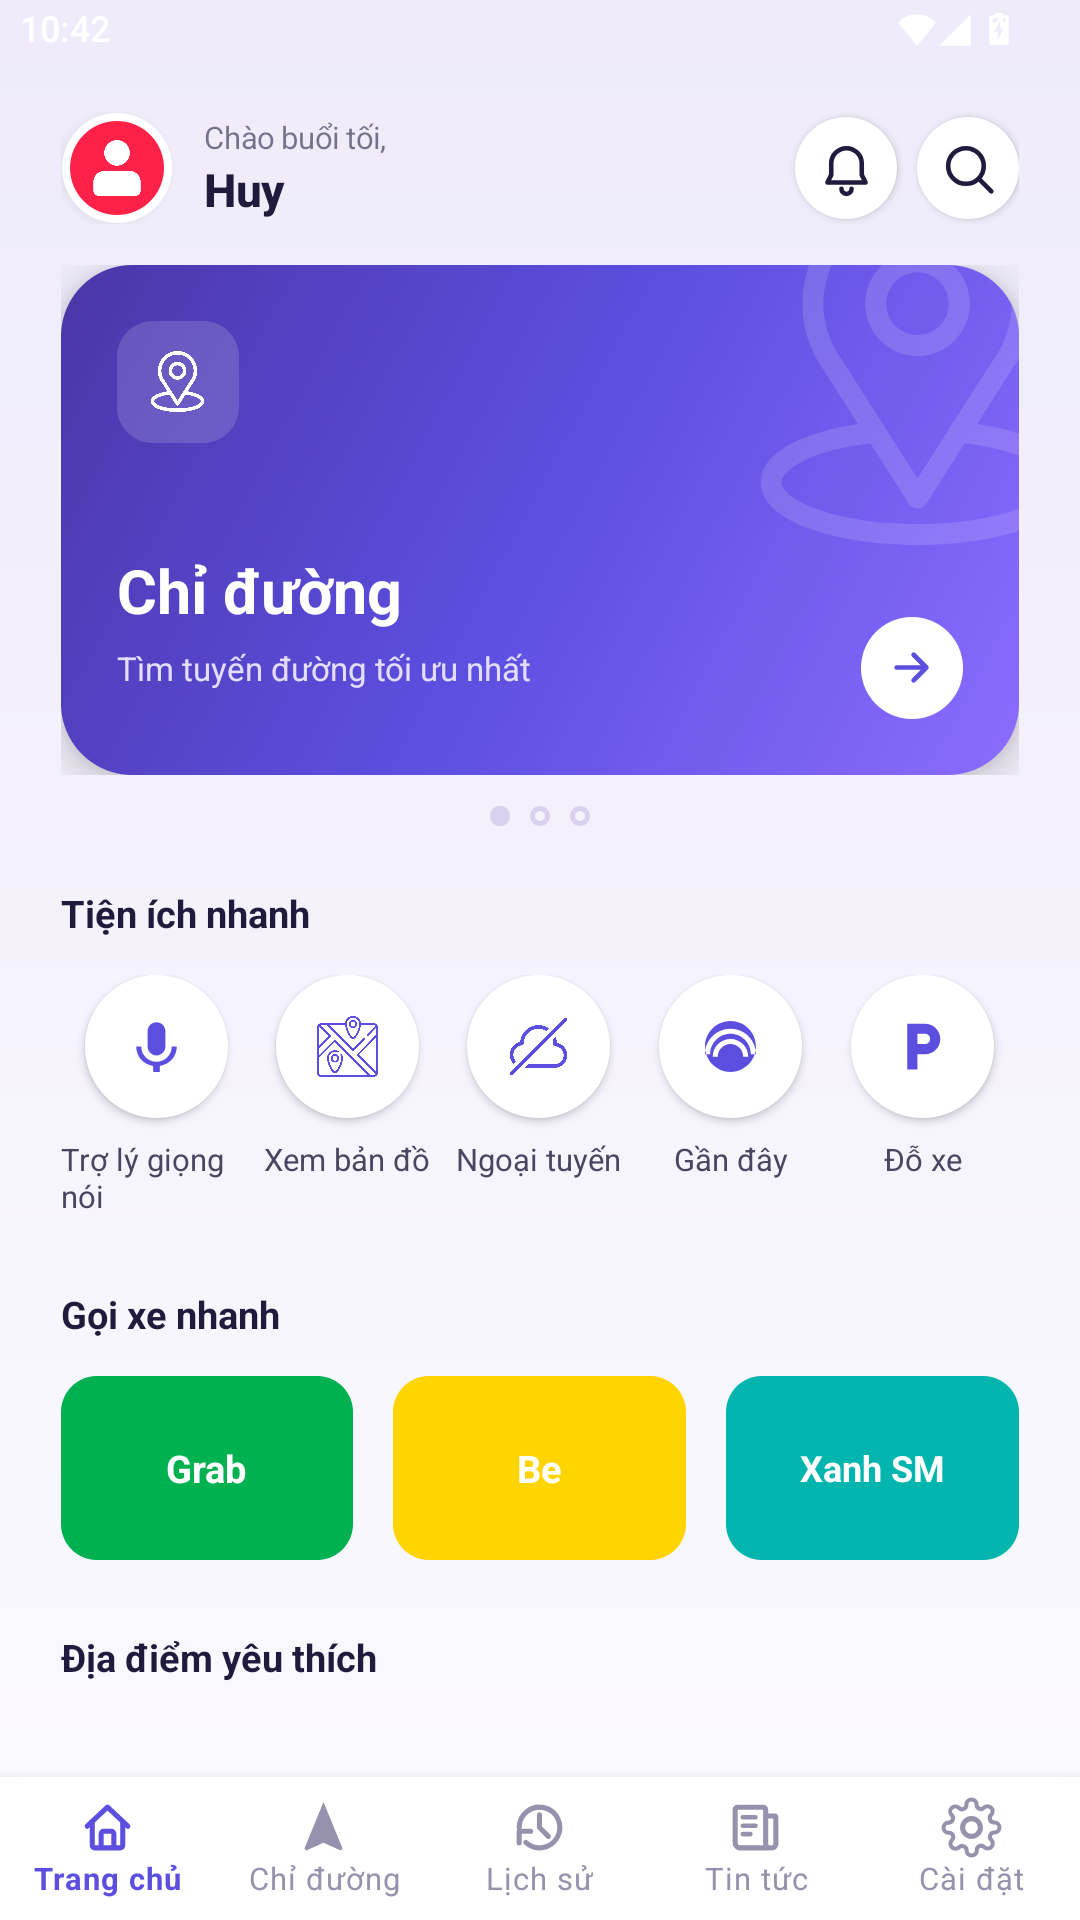
\includegraphics[width=0.72\linewidth]{figures/h15_home_moi.png}
\subcaption{Trang chủ sau khi đồng bộ giao diện}
\end{minipage}\hfill
\begin{minipage}{0.48\textwidth}\centering
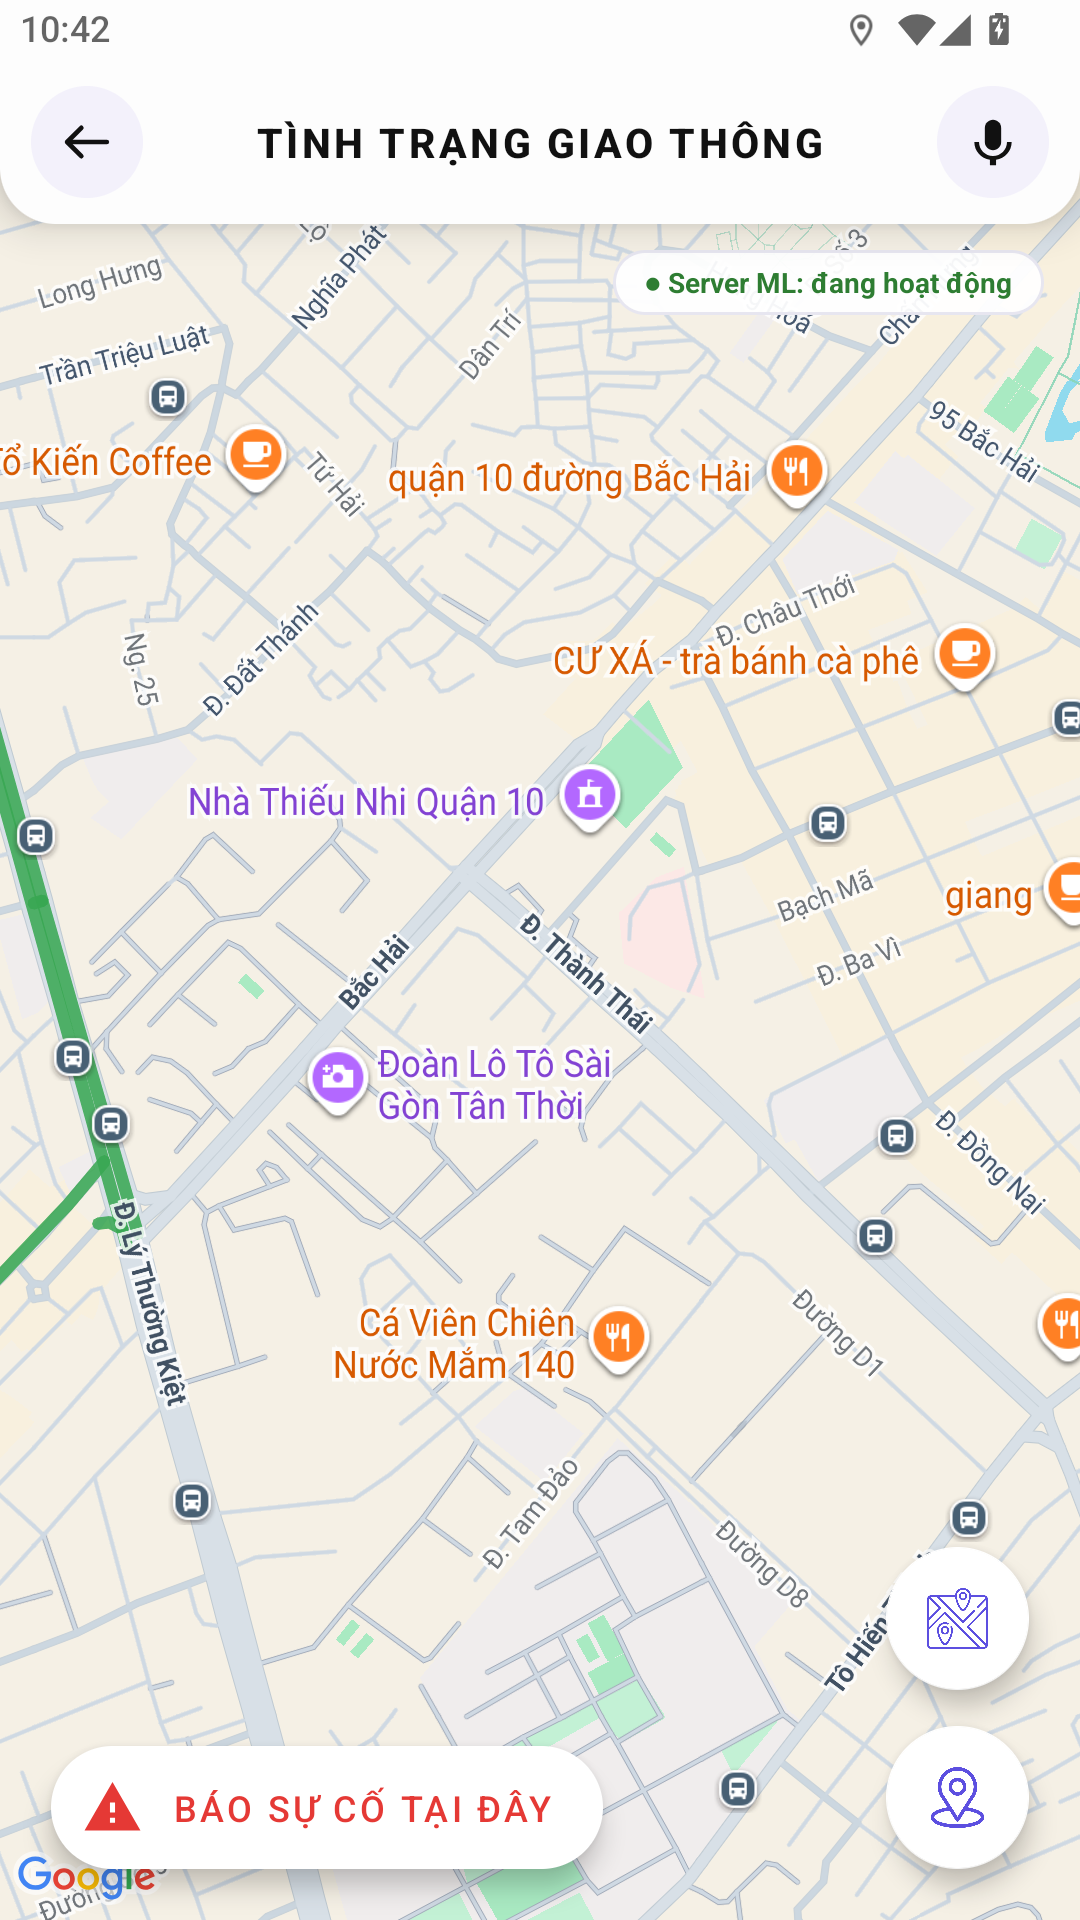
\includegraphics[width=0.72\linewidth]{figures/h16_chip.png}
\subcaption{Chip trạng thái server ML trên bản đồ}
\label{fig:chip}
\end{minipage}
\caption{Phản hồi trạng thái hệ thống cho người dùng.}
\end{figure}

\subsection{Kết quả ứng dụng}
\label{sec:appresults}
Phần này trình bày kết quả hiện thực của ứng dụng TraffiGo qua các màn hình chính, tất cả được chụp trực tiếp trên trình giả lập với giao diện tiếng Việt.

\textbf{Khởi động và đăng nhập.} Ứng dụng mở bằng màn hình onboarding ba trang giới thiệu (Hình~\ref{fig:onboard}) với nút ``Bỏ qua'' đưa thẳng tới đăng nhập; màn đăng nhập (Hình~\ref{fig:login}) hỗ trợ email/mật khẩu và Google Sign-In qua Firebase Authentication --- toàn bộ luồng đã được kiểm chứng end-to-end với tài khoản thực.

\begin{figure}[h!]
\centering
\begin{minipage}{0.48\textwidth}\centering
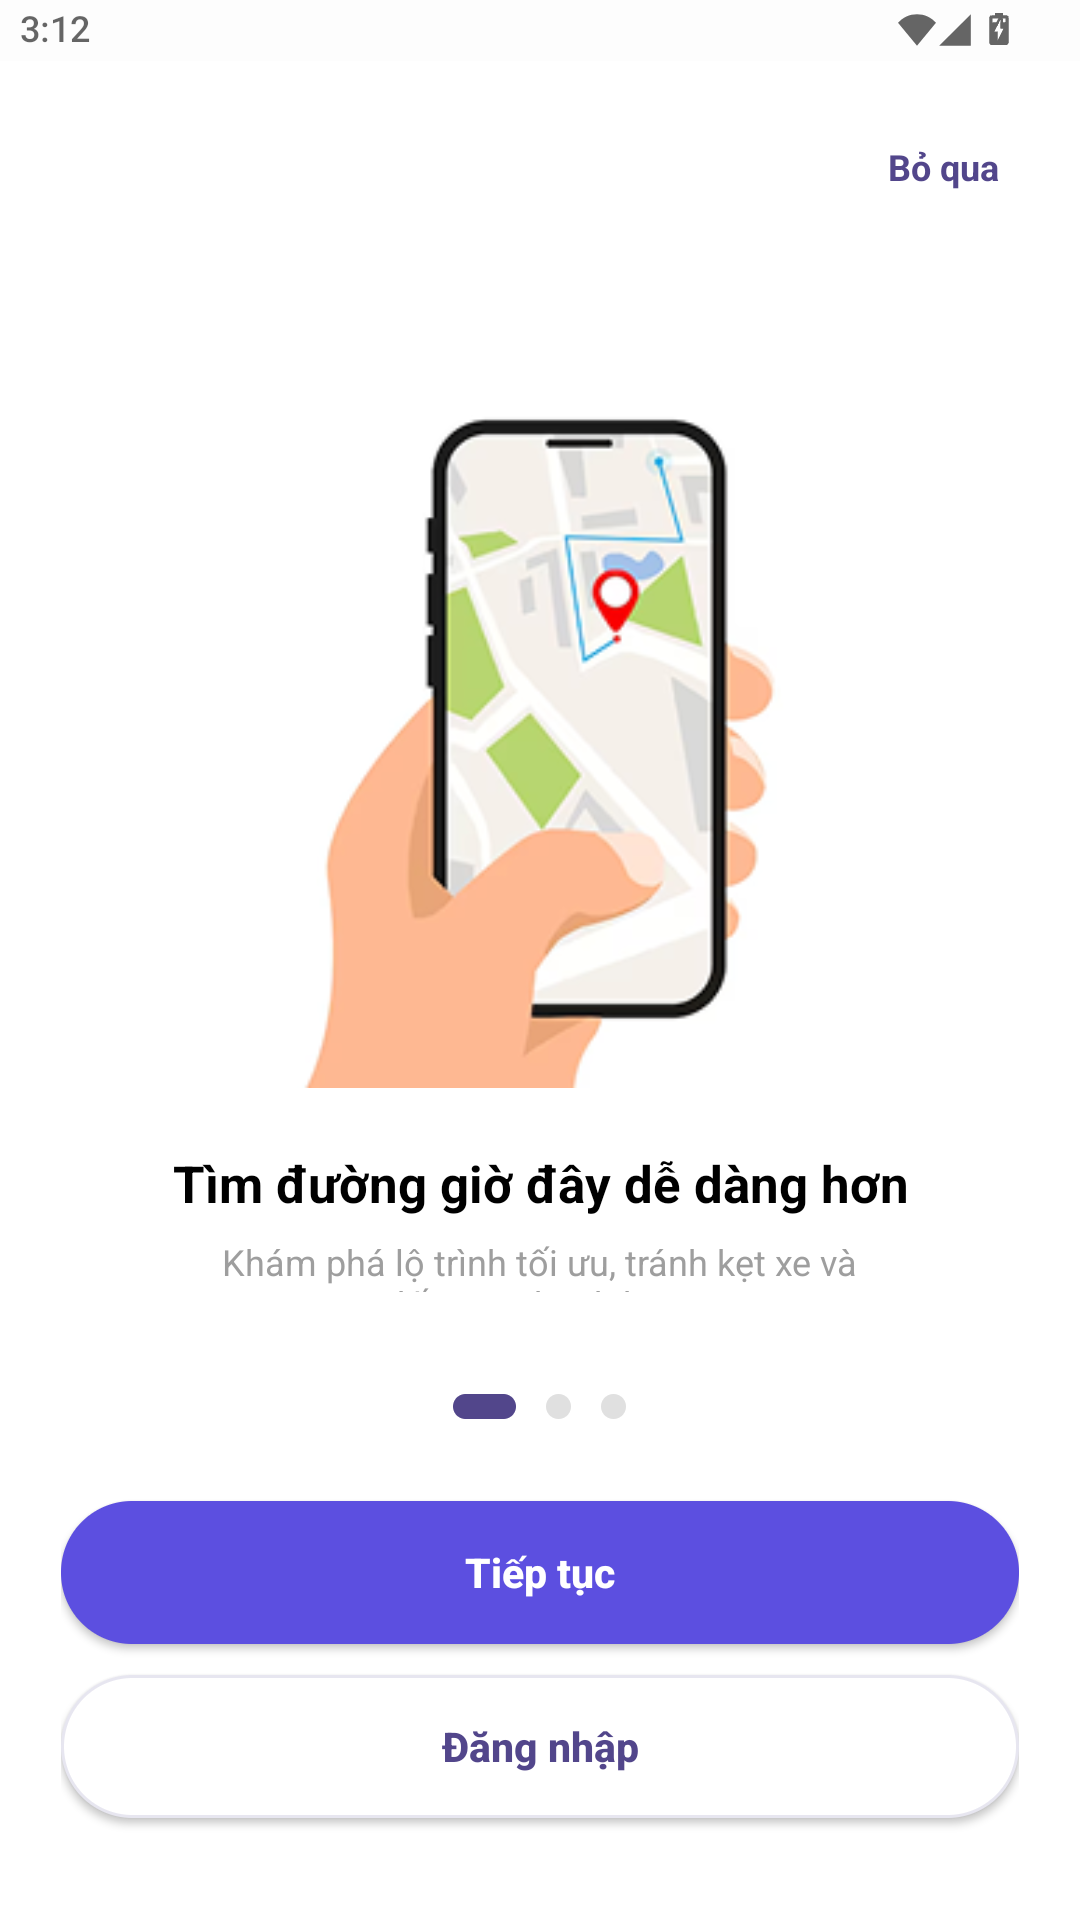
\includegraphics[width=0.72\linewidth]{figures/h01_dangnhapmo.png}
\subcaption{Onboarding}
\label{fig:onboard}
\end{minipage}\hfill
\begin{minipage}{0.48\textwidth}\centering

\includegraphics[width=0.72\linewidth]{figures/h02_dangnhap.png}
\subcaption{Đăng nhập}
\label{fig:login}
\end{minipage}
\caption{Luồng khởi động và đăng nhập của ứng dụng.}
\end{figure}

\textbf{Trang chủ.} Hình~\ref{fig:home} trình bày hub trung tâm với carousel chỉ đường (Chỉ đường / Về nhà / Đến công ty), hàng tiện ích nhanh (trợ lý giọng nói, bản đồ, ngoại tuyến, gần đây, đỗ xe), gọi xe nhanh tới Grab/Be/Xanh SM và danh sách địa điểm yêu thích; thanh điều hướng dưới dẫn tới bốn nhóm chức năng chính.

\begin{figure}[h!]
\centering
\begin{tikzpicture}
\node[anchor=north west,inner sep=0] (home) at (0,0)
 {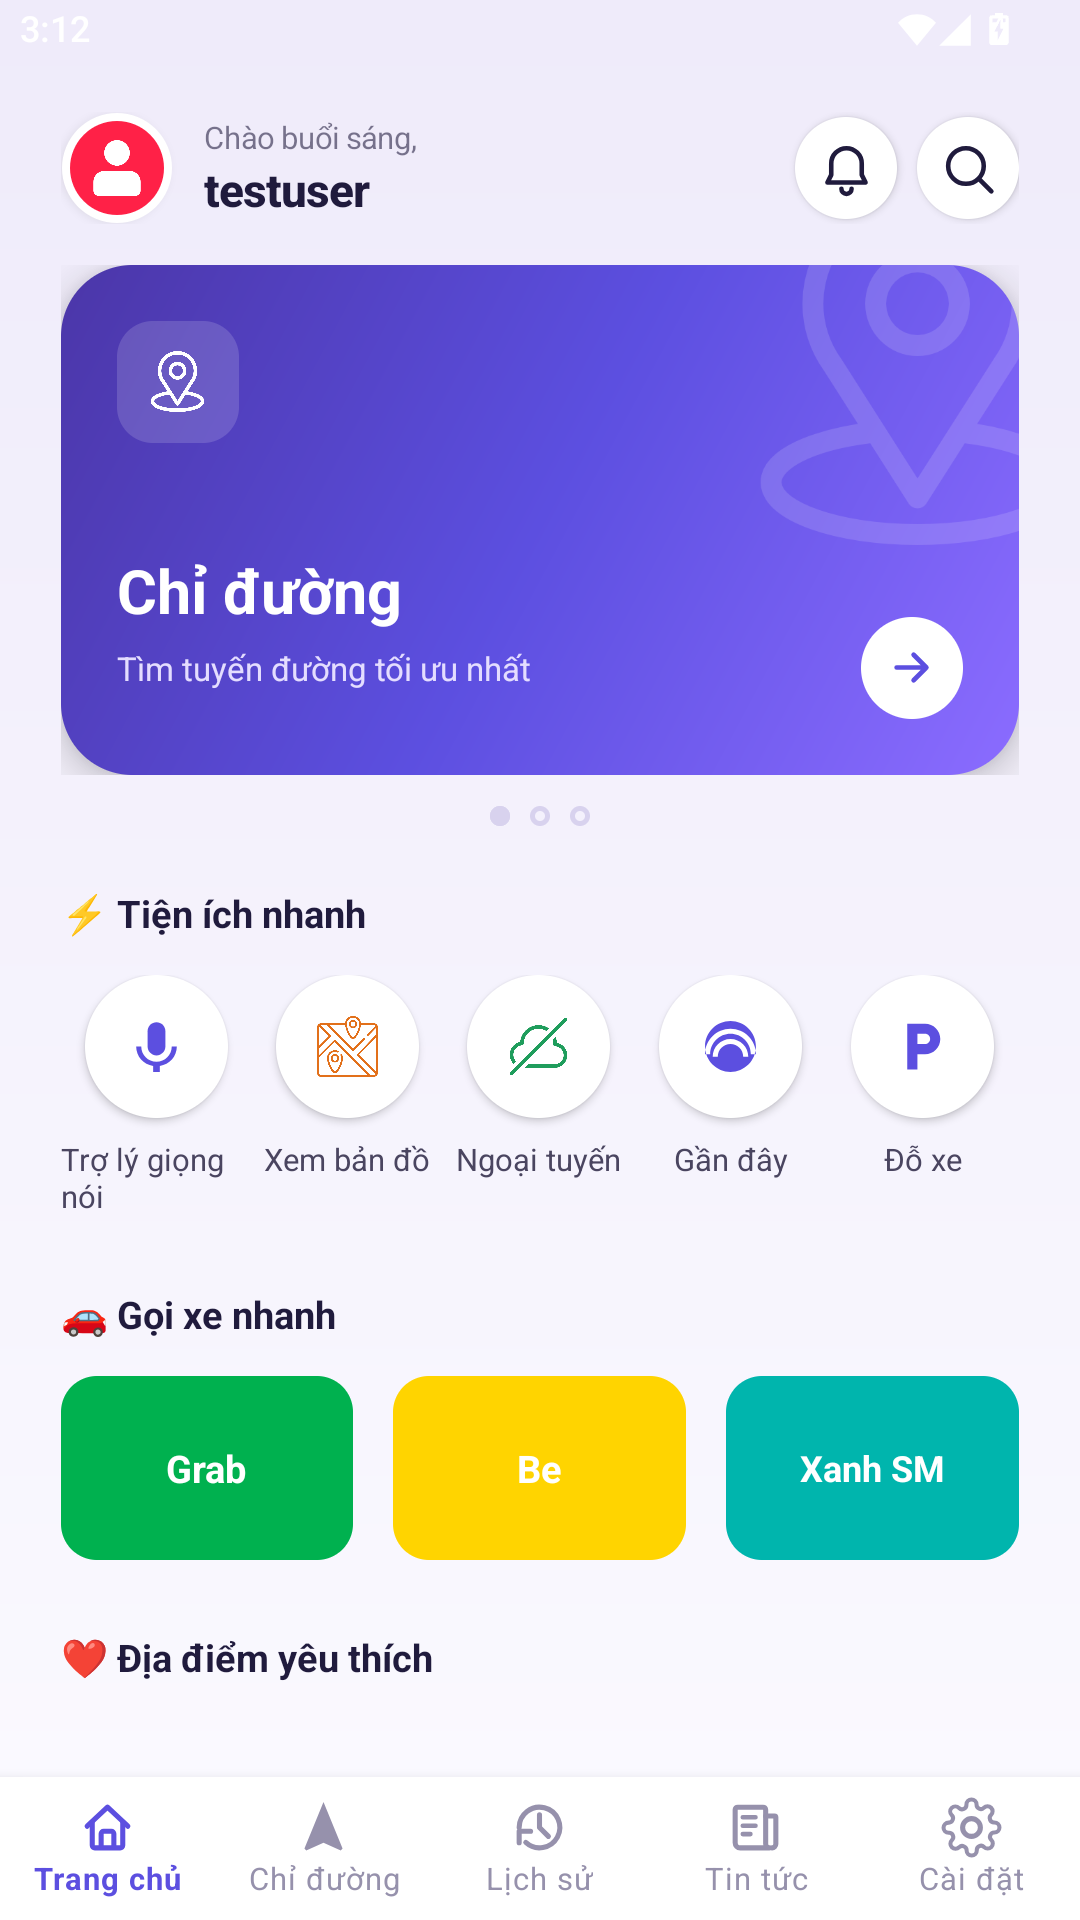
\includegraphics[width=0.56\textwidth]{figures/h03_trangchu.png}};
\fill[screenbg] ([xshift=42pt,yshift=-30pt]home.north west)
 rectangle ([xshift=110pt,yshift=-50pt]home.north west);
\node[anchor=west,inner sep=0,font=\sffamily\bfseries\fontsize{10}{12}\selectfont,text=appink]
 at ([xshift=45pt,yshift=-43pt]home.north west) {Quang Huy};
\end{tikzpicture}
\caption{Màn hình Trang chủ của TraffiGo.}
\label{fig:home}
\end{figure}

\textbf{Bản đồ giao thông theo cụm.} Hình~\ref{fig:trafficmap} là màn hình lõi của hệ thống: các đoạn đường được tô màu theo cụm K-Means (xanh = thoáng, đỏ = kẹt) dựa trên dữ liệu live TomTom; đoạn chưa có dữ liệu tô xám. Khi bấm vào một đoạn (Hình~\ref{fig:mlsheet}), bottom sheet hiện tốc độ live và trạng thái, kèm \textbf{thẻ ``Dự báo ML (server)''} --- kết quả tích hợp server: tốc độ dự đoán $\approx$ 28 km/h, mức trung bình, cụm giao thông \#0, rủi ro sự cố THẤP.

\begin{figure}[h!]
\centering
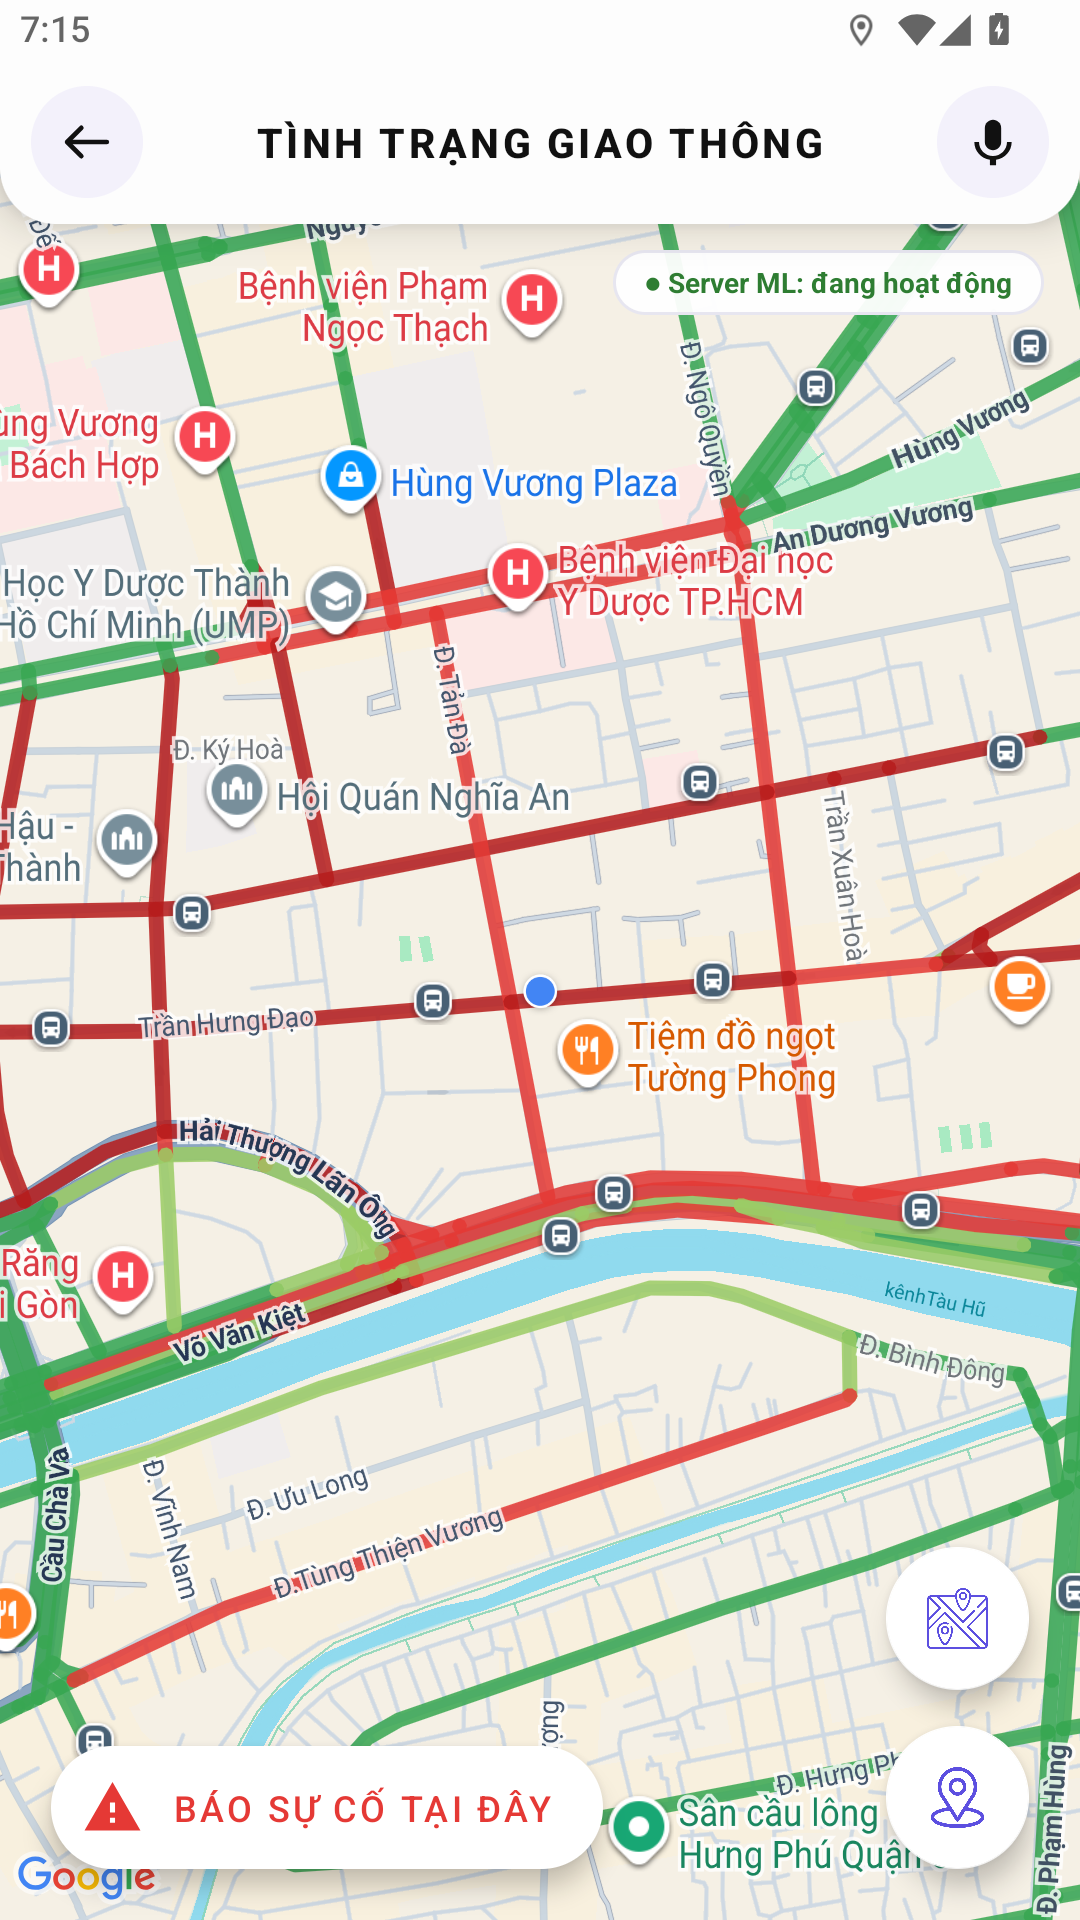
\includegraphics[width=0.56\textwidth]{figures/h04_bandogiaothong.png}
\caption{Bản đồ Tình trạng giao thông: các đoạn tô màu theo cụm K-Means.}
\label{fig:trafficmap}
\end{figure}

\begin{figure}[h!]
\centering
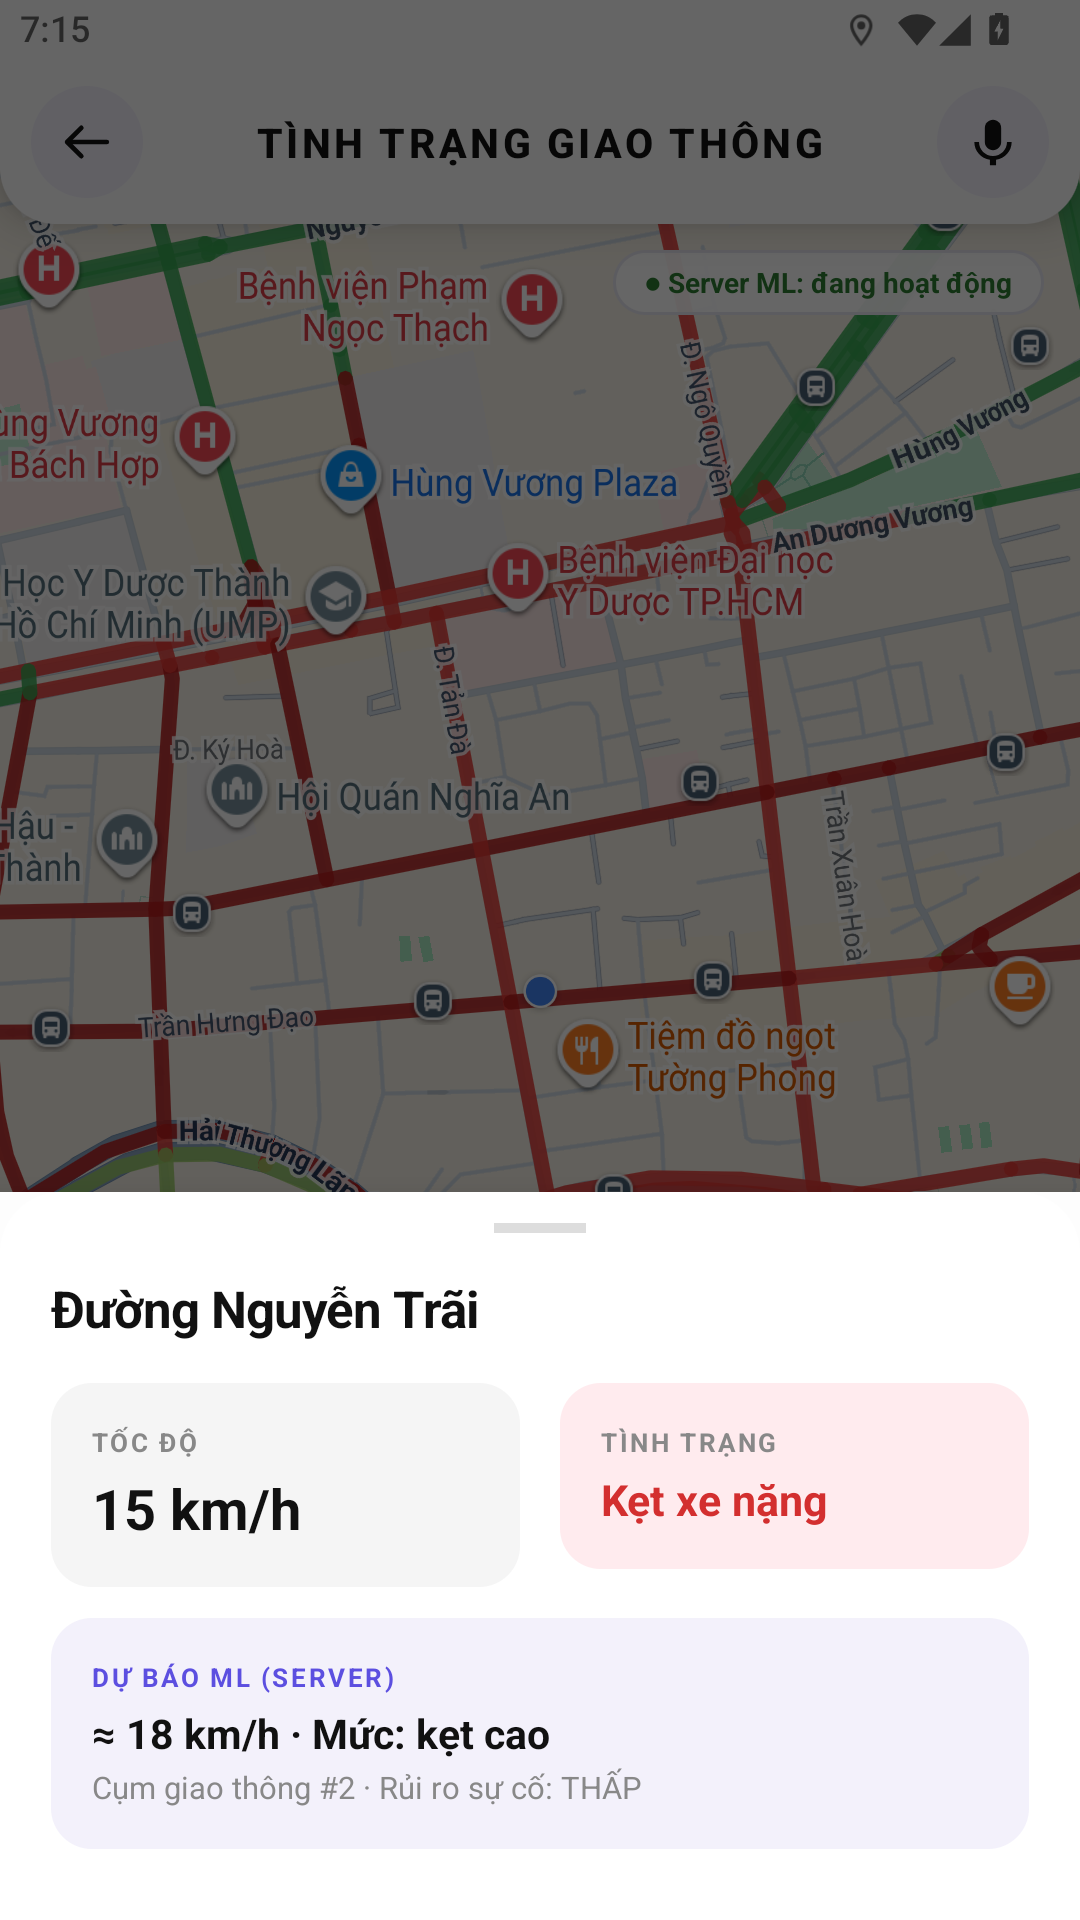
\includegraphics[width=0.56\textwidth]{figures/h05_mldubao.png}
\caption{Bottom sheet chi tiết đoạn với thẻ Dự báo ML từ server.}
\label{fig:mlsheet}
\end{figure}

\textbf{Chỉ đường né kẹt.} Luồng tìm đường bắt đầu từ màn ``Bắt đầu hành trình'' (Hình~\ref{fig:lotrinh}): điểm đi mặc định là vị trí GPS hiện tại (đã reverse-geocode sang địa chỉ tiếng Việt), có thể chọn ``Vị trí hiện tại'', nhà/công ty đã lưu hoặc chạm bản đồ; chọn phương tiện ô tô/xe máy/đi bộ và tùy chọn tránh phí (Hình~\ref{fig:diemden} --- hỗ trợ thêm điểm dừng trung gian).

\begin{figure}[h!]
\centering
\begin{minipage}{0.48\textwidth}\centering
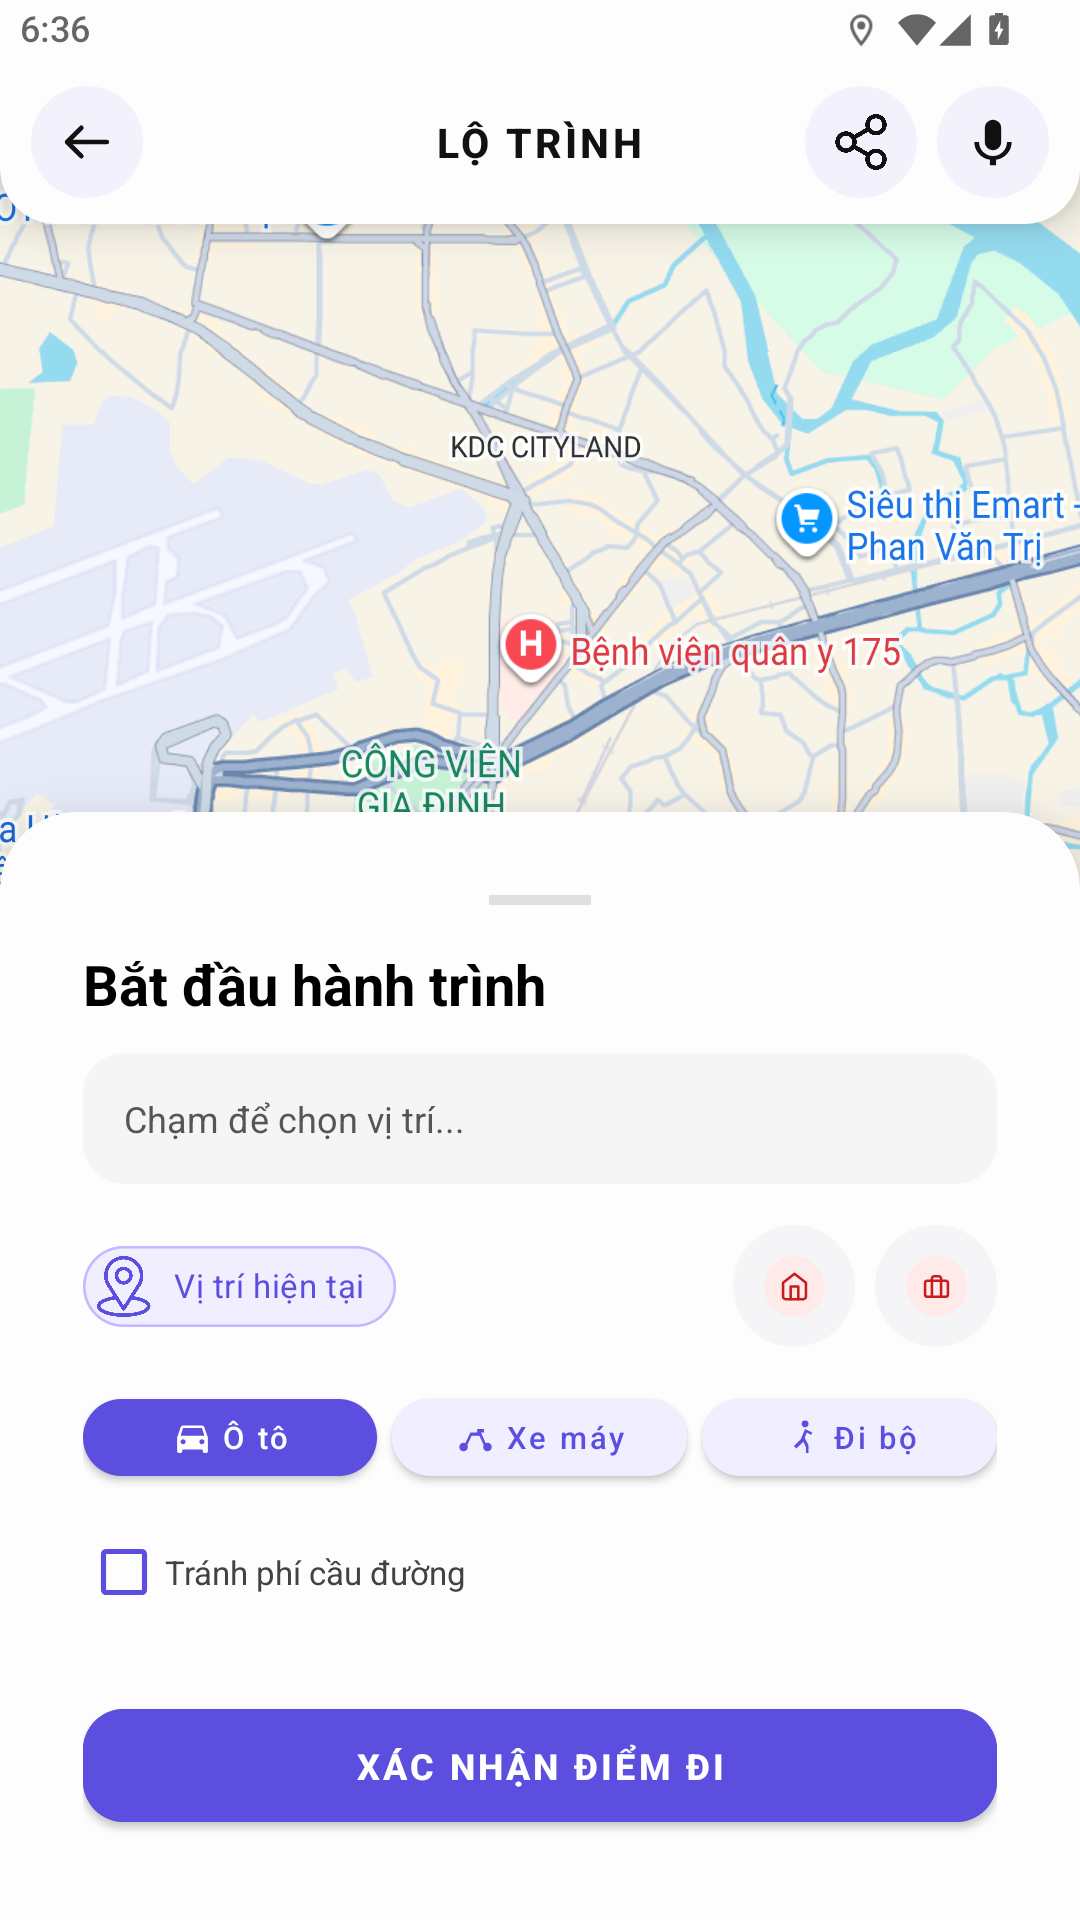
\includegraphics[width=0.72\linewidth]{figures/h08_lotrinh.png}
\subcaption{Bắt đầu hành trình}
\label{fig:lotrinh}
\end{minipage}\hfill
\begin{minipage}{0.48\textwidth}\centering
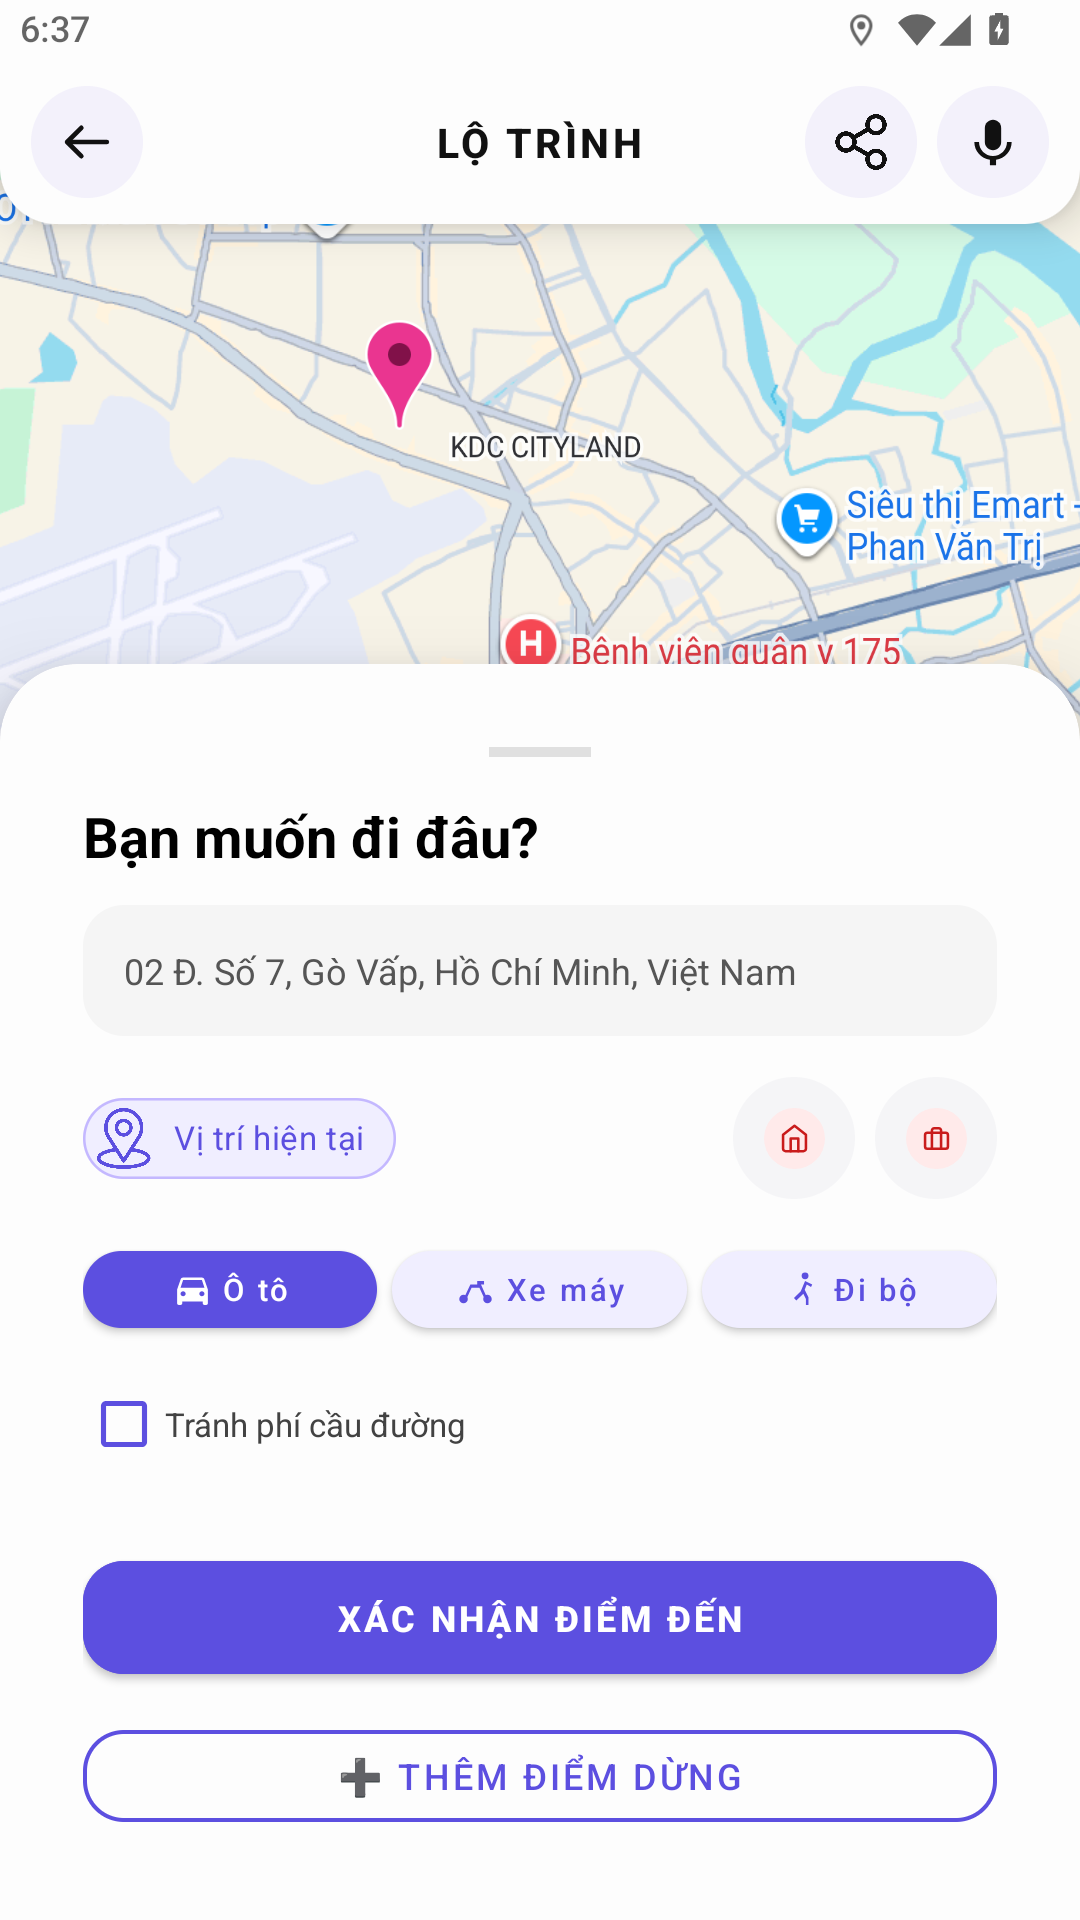
\includegraphics[width=0.72\linewidth]{figures/h10_diemden.png}
\subcaption{Chọn điểm đến, thêm điểm dừng}
\label{fig:diemden}
\end{minipage}
\caption{Luồng chọn điểm đi --- điểm đến.}
\end{figure}

Hình~\ref{fig:routeinfo} thể hiện kết quả chấm điểm tuyến: với tuyến 16 phút/5,7 km, hệ thống phát hiện \textbf{đoạn tắc nghẽn nặng} trên tuyến và cảnh báo ``ước tính thêm $\sim$25 phút'', gán \textbf{sức khỏe tuyến F}; dòng ``TraffiGo chọn tuyến ít tắc hơn tuyến nhanh nhất của Google'' xuất hiện khi thuật toán chọn tuyến dài hơn nhưng thông thoáng hơn dựa trên trọng số phạt kẹt~\eqref{eq:penalty} --- minh chứng trực quan cho giá trị của kết quả gom cụm trong định tuyến.

\begin{figure}[h!]
\centering
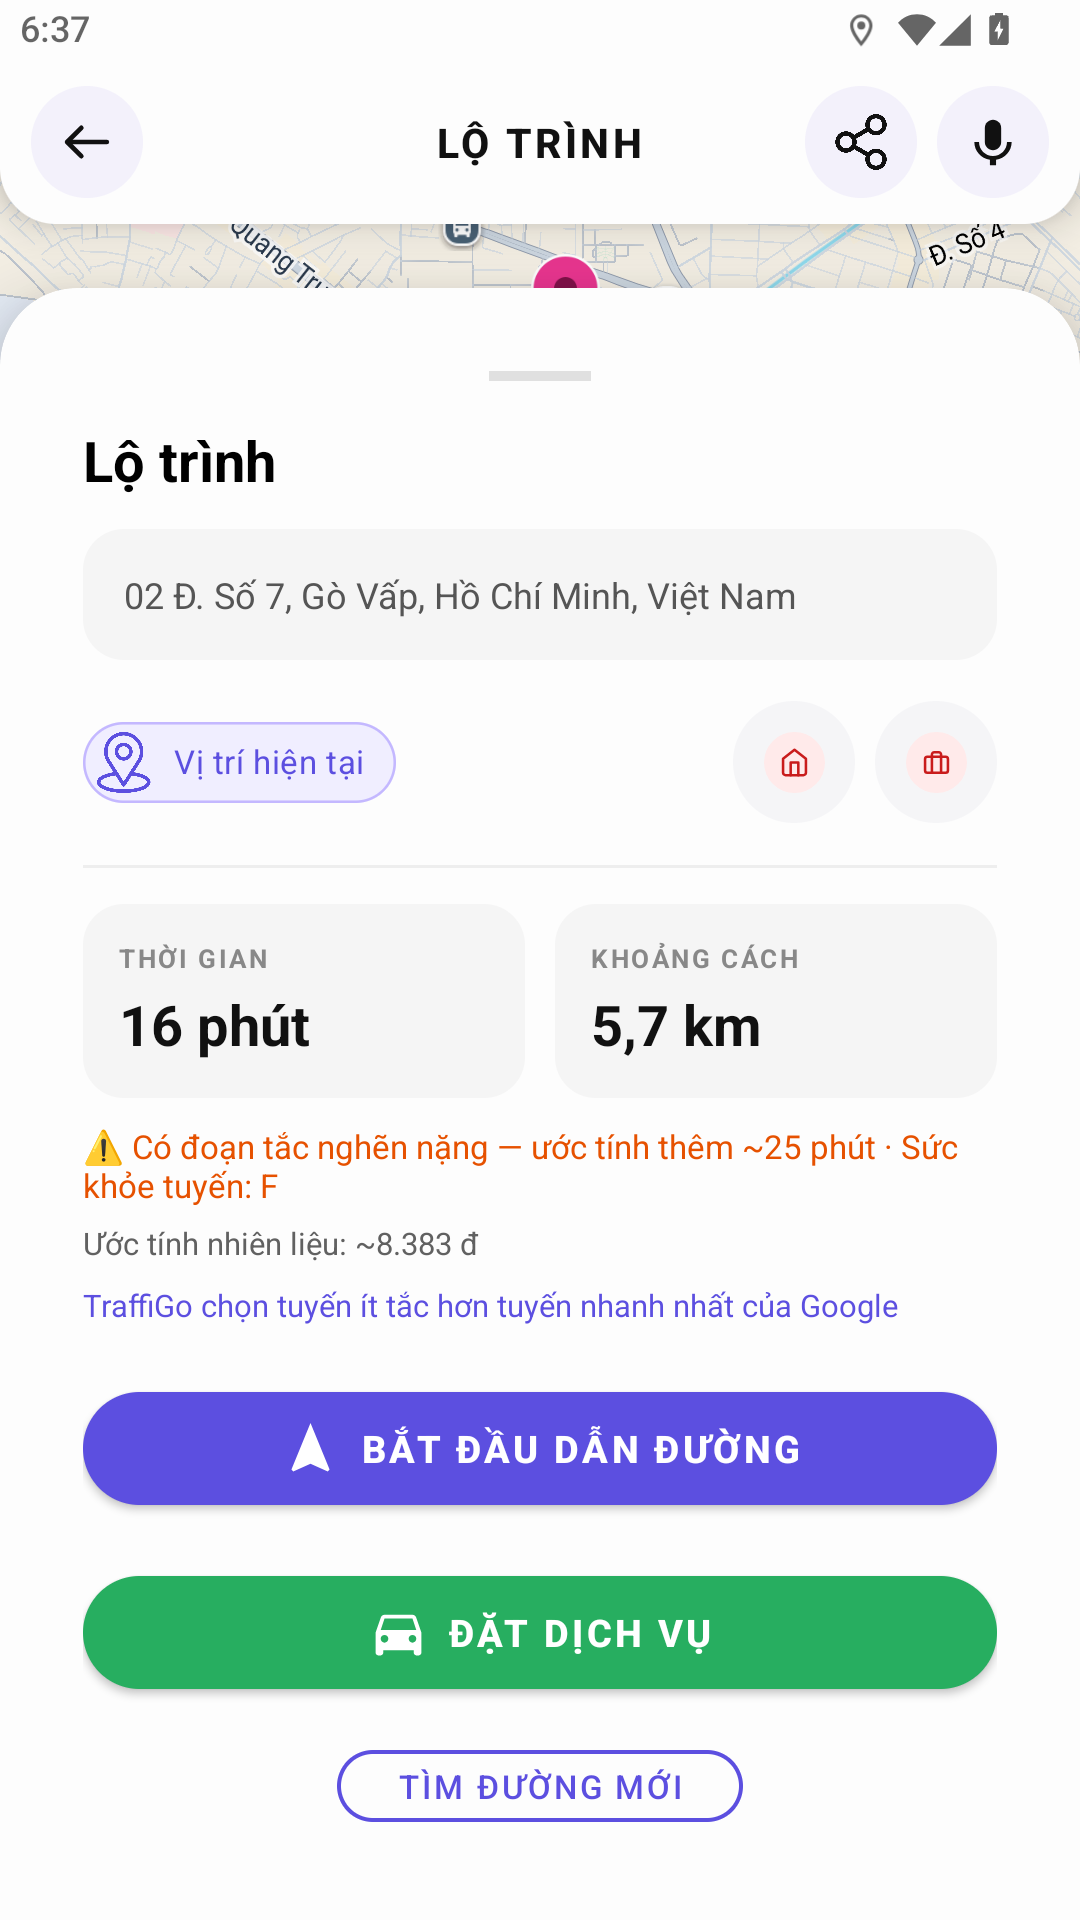
\includegraphics[width=0.56\textwidth]{figures/h11_thongtinlo.png}
\caption{Thông tin tuyến: thời gian, quãng đường, cảnh báo tắc, sức khỏe tuyến, ước tính nhiên liệu.}
\label{fig:routeinfo}
\end{figure}

\begin{figure}[h!]
\centering
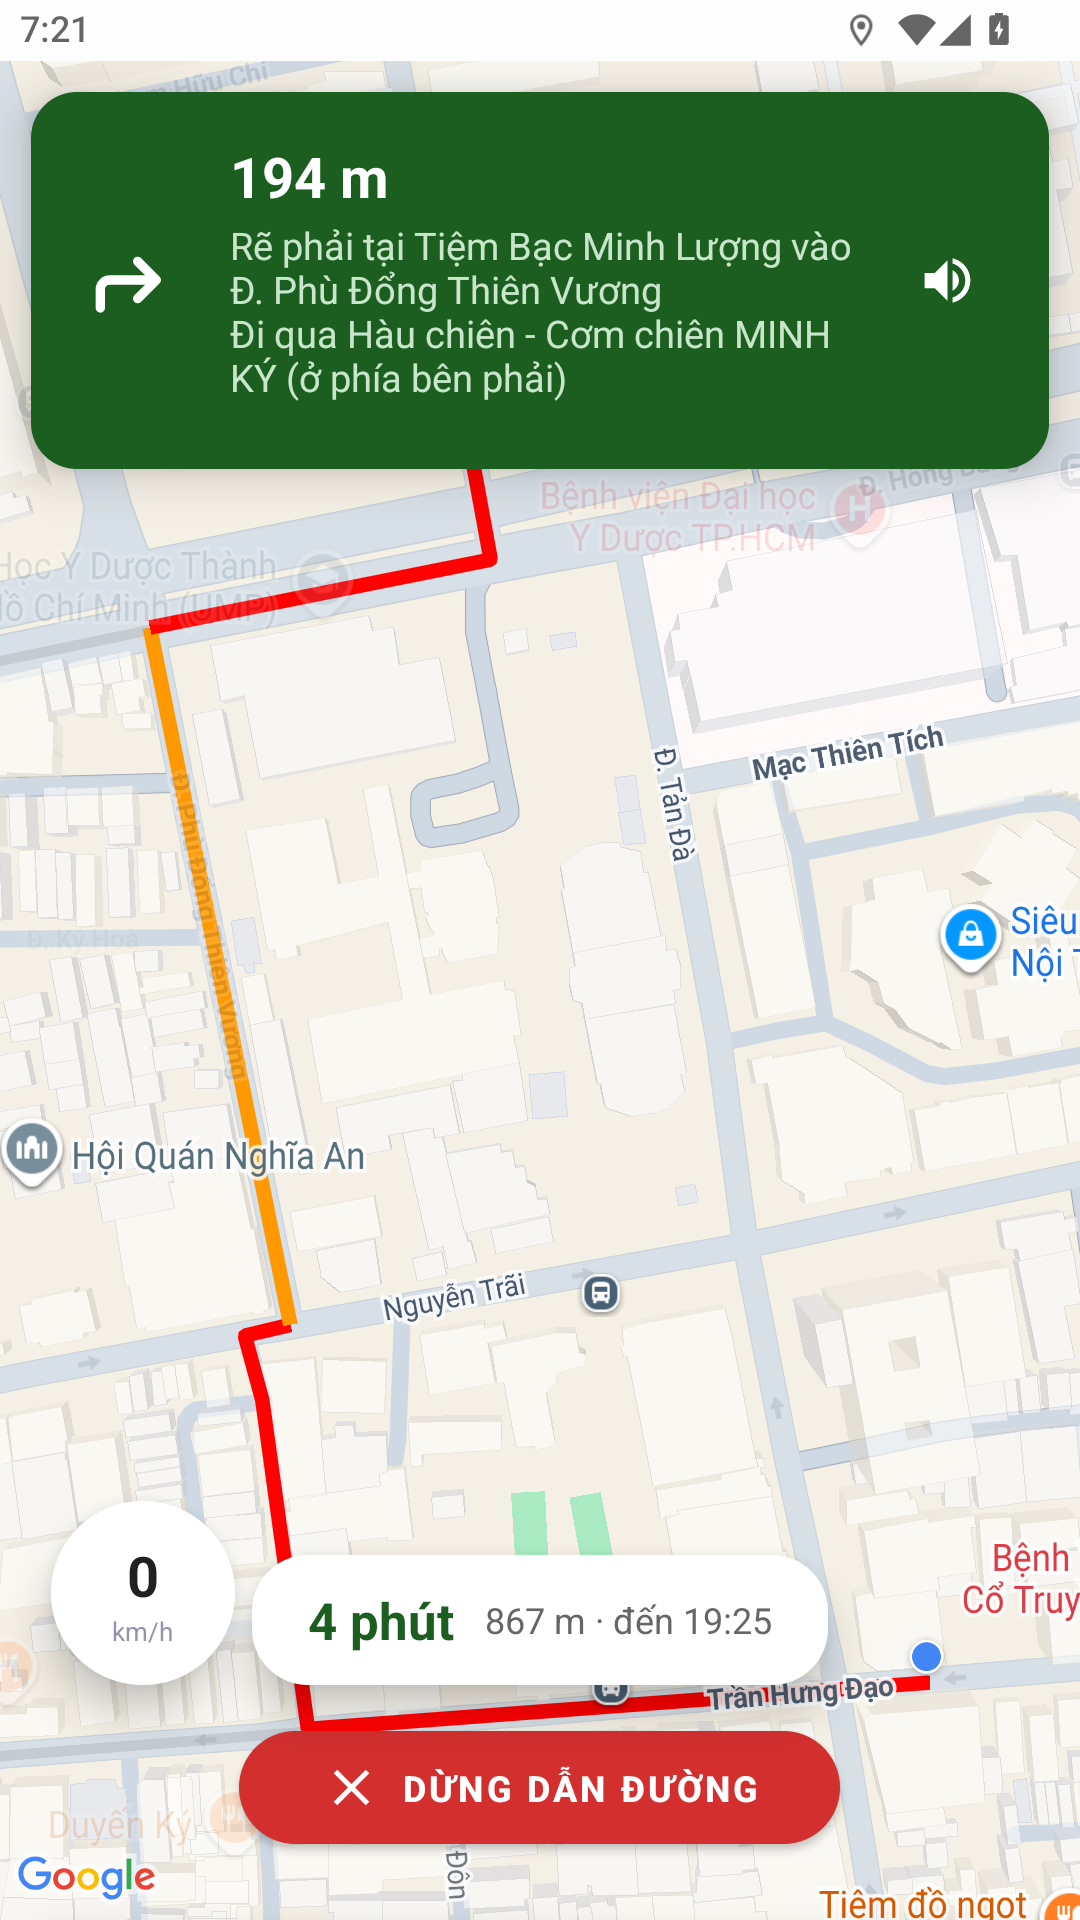
\includegraphics[width=0.56\textwidth]{figures/h17_danhuong.png}
\caption{Chế độ điều hướng turn-by-turn: banner hướng dẫn rẽ, đồng hồ tốc độ, tuyến tô màu theo cụm và thời gian đến đích.}
\label{fig:nav}
\end{figure}

Khi chế độ điều hướng khởi động, camera bám theo vị trí GPS của người dùng, banner phía trên hiển thị maneuvre kế tiếp kèm khoảng cách và ghi chú địa điểm đi qua (``Rẽ phải tại Tiệm Bạc Minh Lượng vào Đ. Phù Đổng Thiên Vương''), đồng hồ tốc độ ở góc trái, và nút dừng dẫn đường luôn trong tầm tay (Hình~\ref{fig:nav}). Trong suốt hành trình, tuyến đường phía sau được tô lại màu theo cụm giao thông cập nhật.

\textbf{Tin tức và địa điểm lân cận.} Hình~\ref{fig:news} tổng hợp tin giao thông từ năm báo điện tử (VnExpress, Thanh Niên, Tuổi Trẻ, Dân Trí, VietNamNet) với chip lọc danh mục; bài viết có thể được đọc to bằng TTS với tốc độ điều chỉnh. Hình~\ref{fig:nearby} tìm địa điểm quanh vị trí GPS theo danh mục (Xăng, ATM, Ăn uống, Bệnh viện...) với khoảng cách thực tế.

\begin{figure}[h!]
\centering
\begin{minipage}{0.48\textwidth}\centering
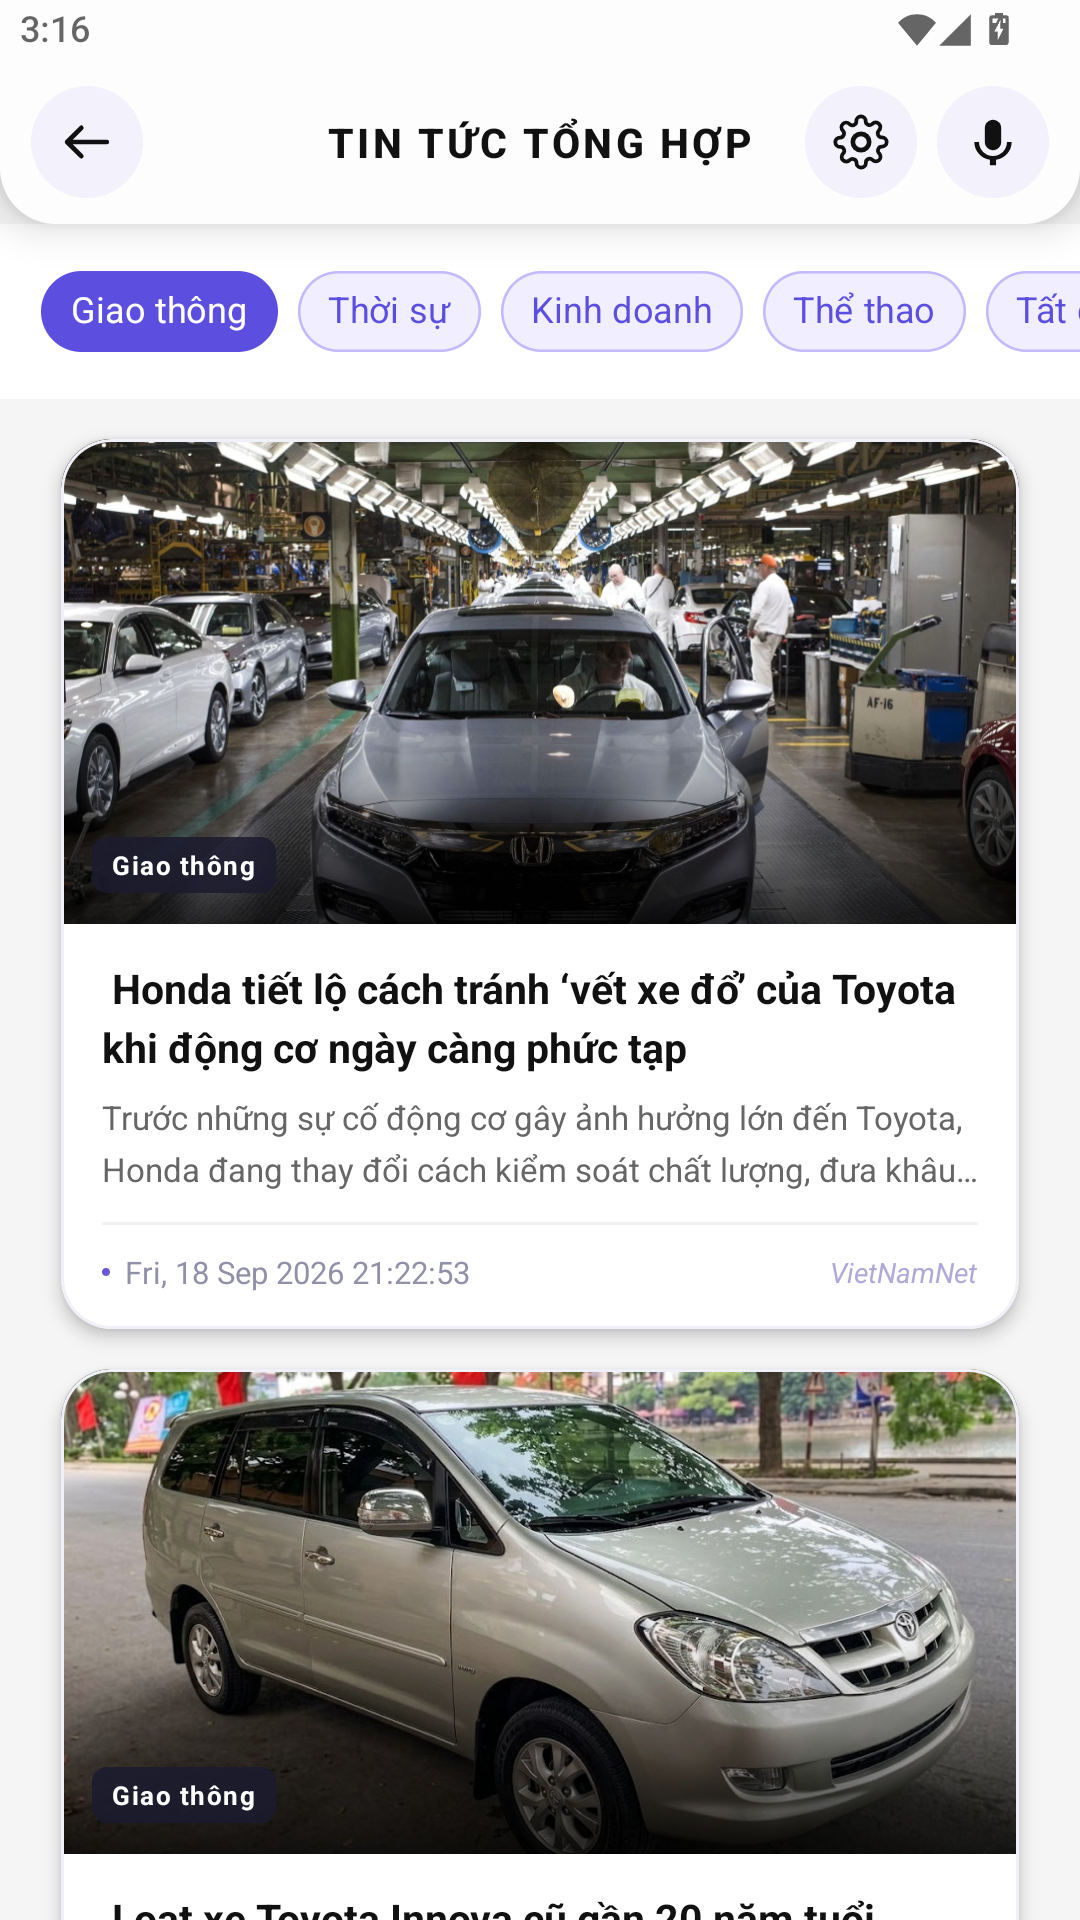
\includegraphics[width=0.72\linewidth]{figures/h06_tintuc.png}
\subcaption{Tin tức tổng hợp}
\label{fig:news}
\end{minipage}\hfill
\begin{minipage}{0.48\textwidth}\centering
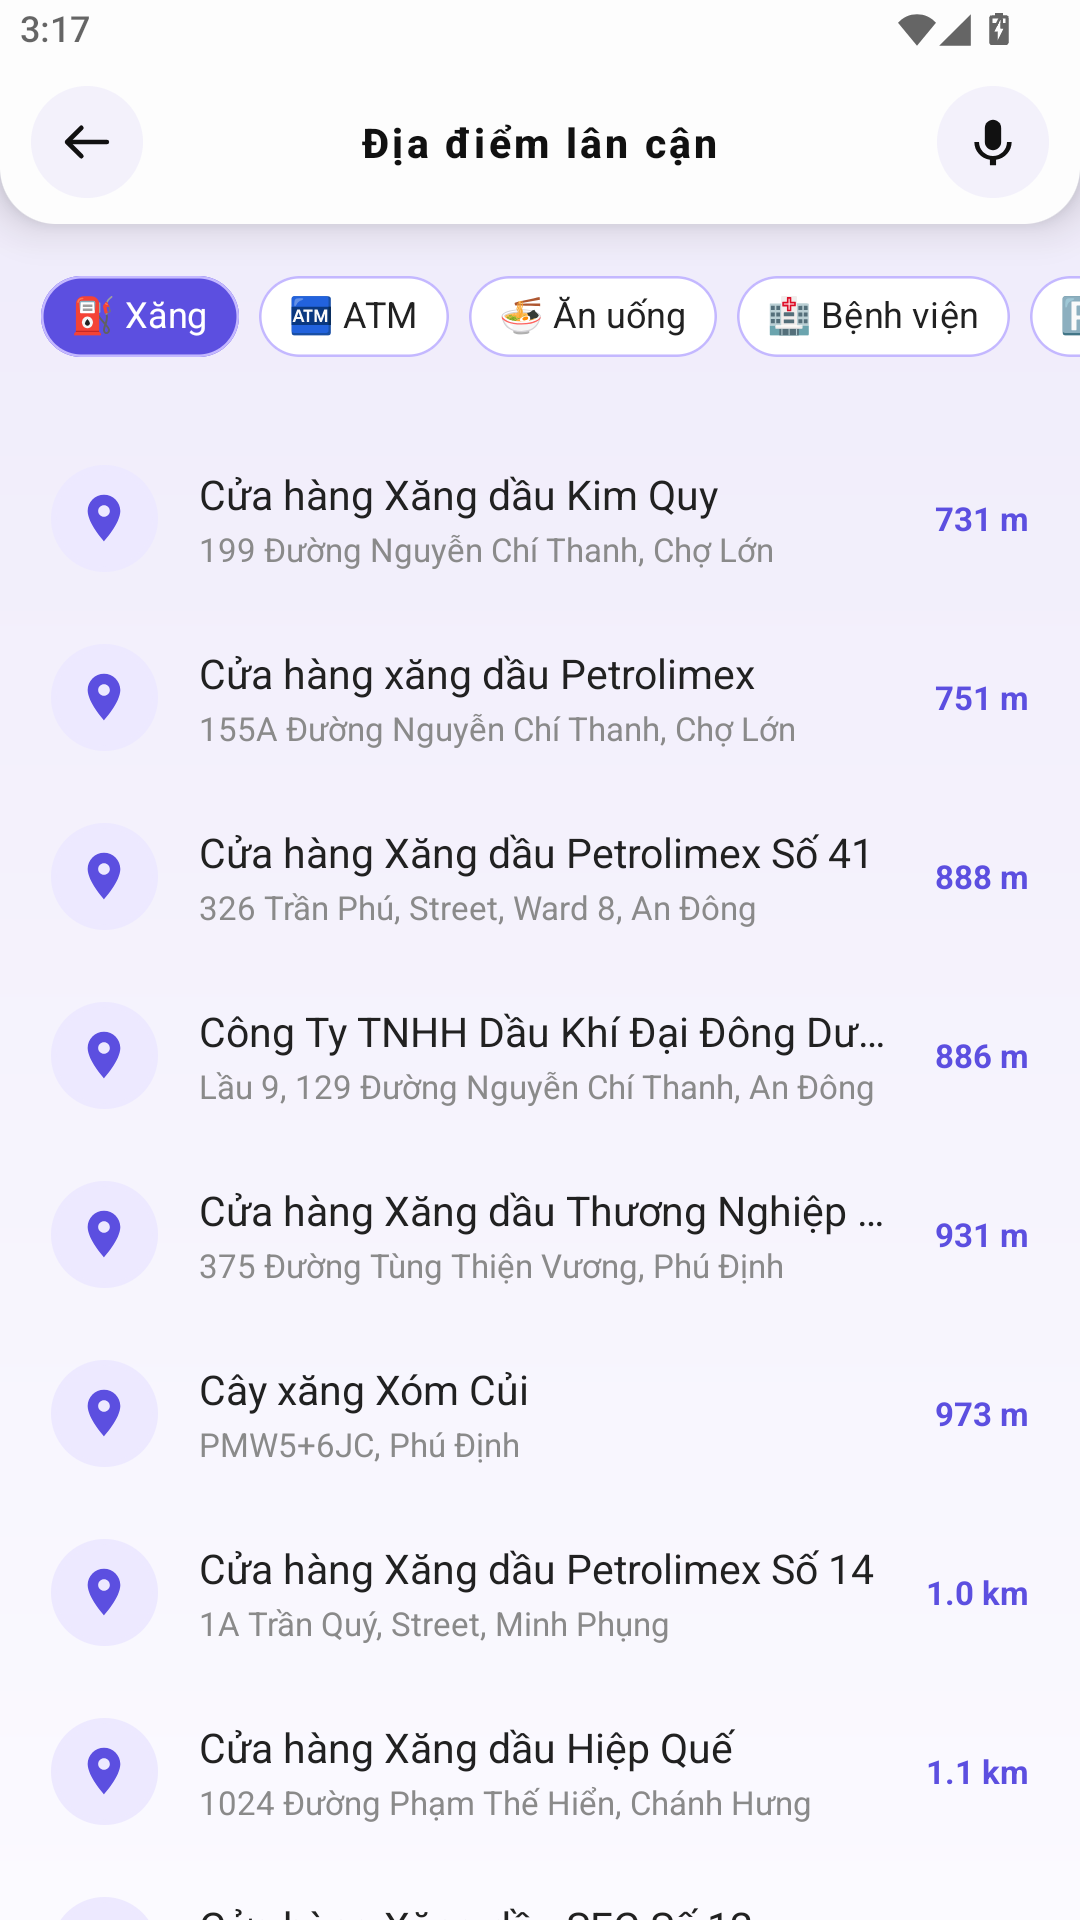
\includegraphics[width=0.72\linewidth]{figures/h07_gancanh.png}
\subcaption{Địa điểm lân cận}
\label{fig:nearby}
\end{minipage}
\caption{Tin tức giao thông và tìm địa điểm lân cận.}
\end{figure}

\textbf{Hồ sơ, lịch sử và bản đồ ngoại tuyến.} Hình~\ref{fig:profile} quản lý thông tin cá nhân (tên, số điện thoại, avatar lưu Base64 vào Realtime Database); Hình~\ref{fig:history} lưu lại các chuyến đi để \textit{trải lại tuyến này} chỉ với một chạm; Hình~\ref{fig:offline} là danh sách vùng bản đồ đã lưu (tên, ngày lưu, dung lượng) dùng khi không có kết nối mạng.

\begin{figure}[h!]
\centering
\begin{minipage}{0.32\textwidth}\centering
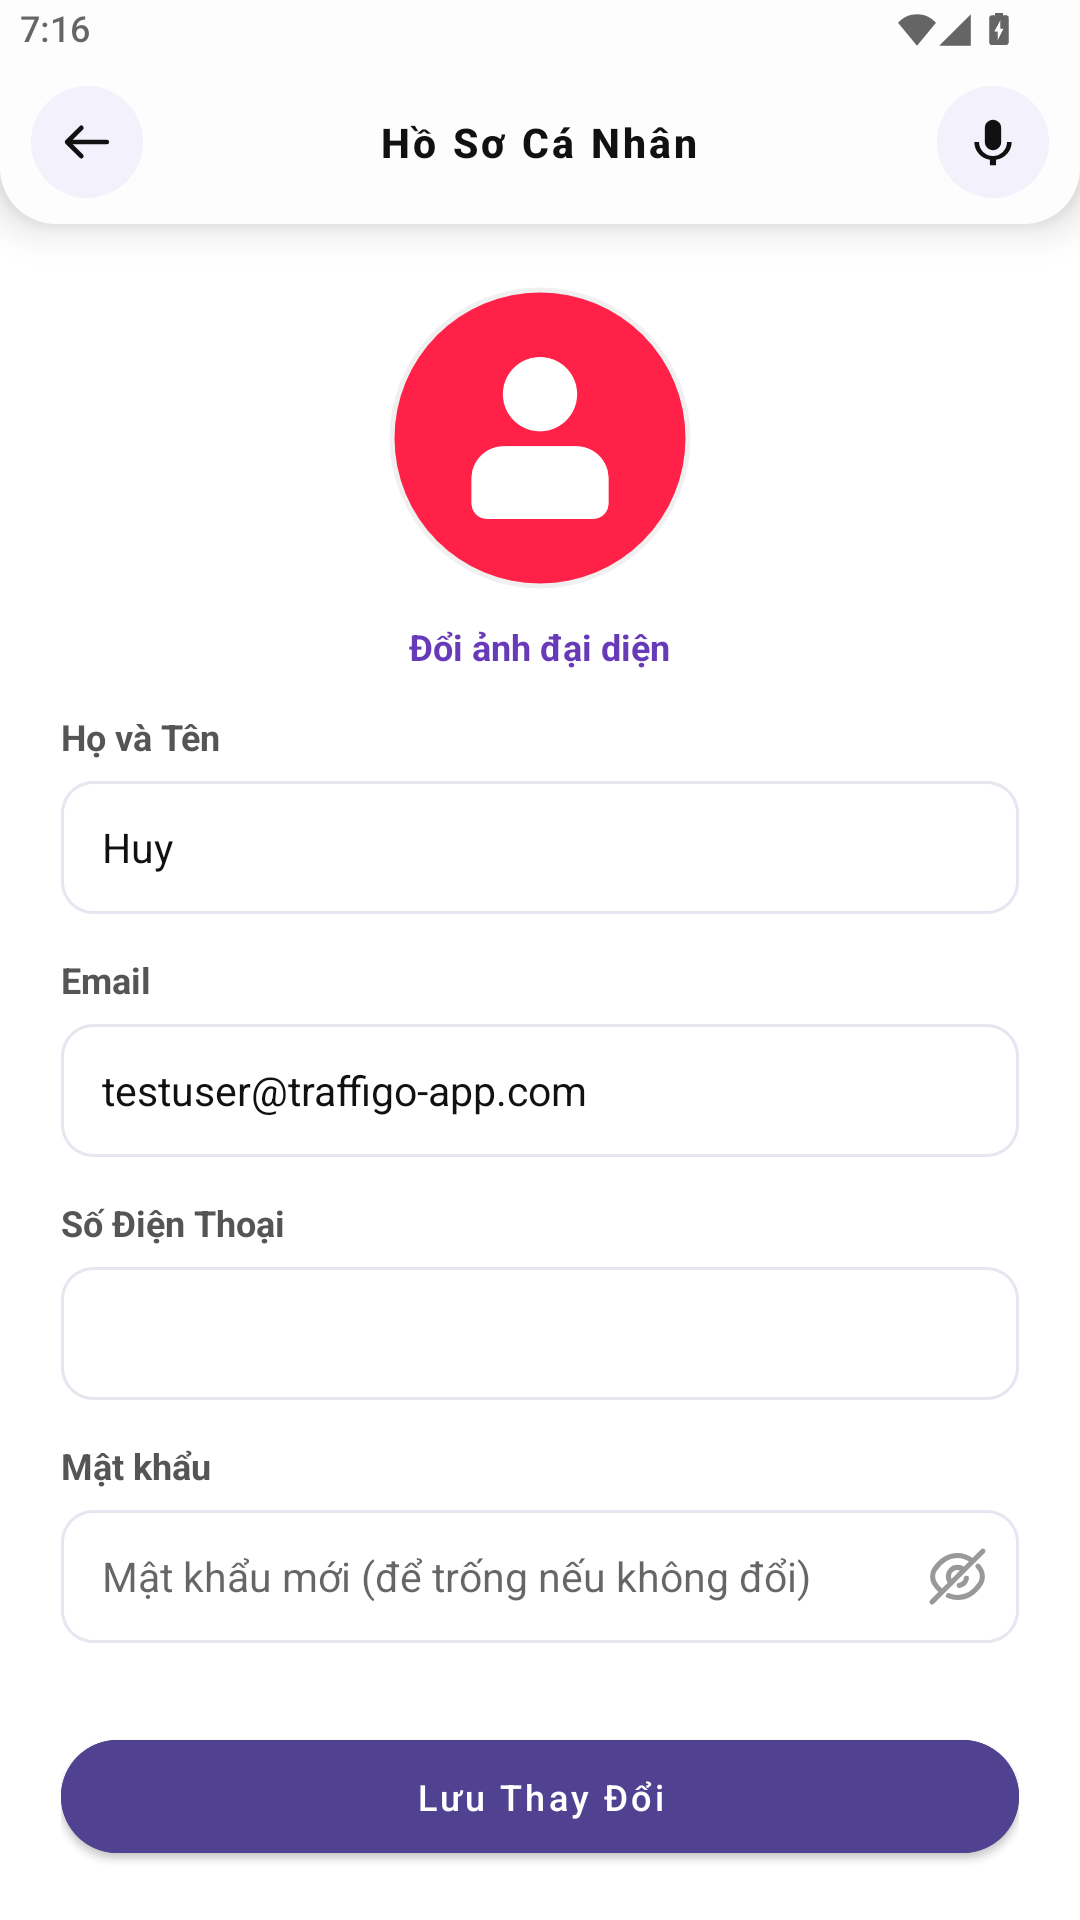
\includegraphics[width=0.9\linewidth]{figures/h12_hoso.png}
\subcaption{Hồ sơ cá nhân}
\label{fig:profile}
\end{minipage}\hfill
\begin{minipage}{0.32\textwidth}\centering
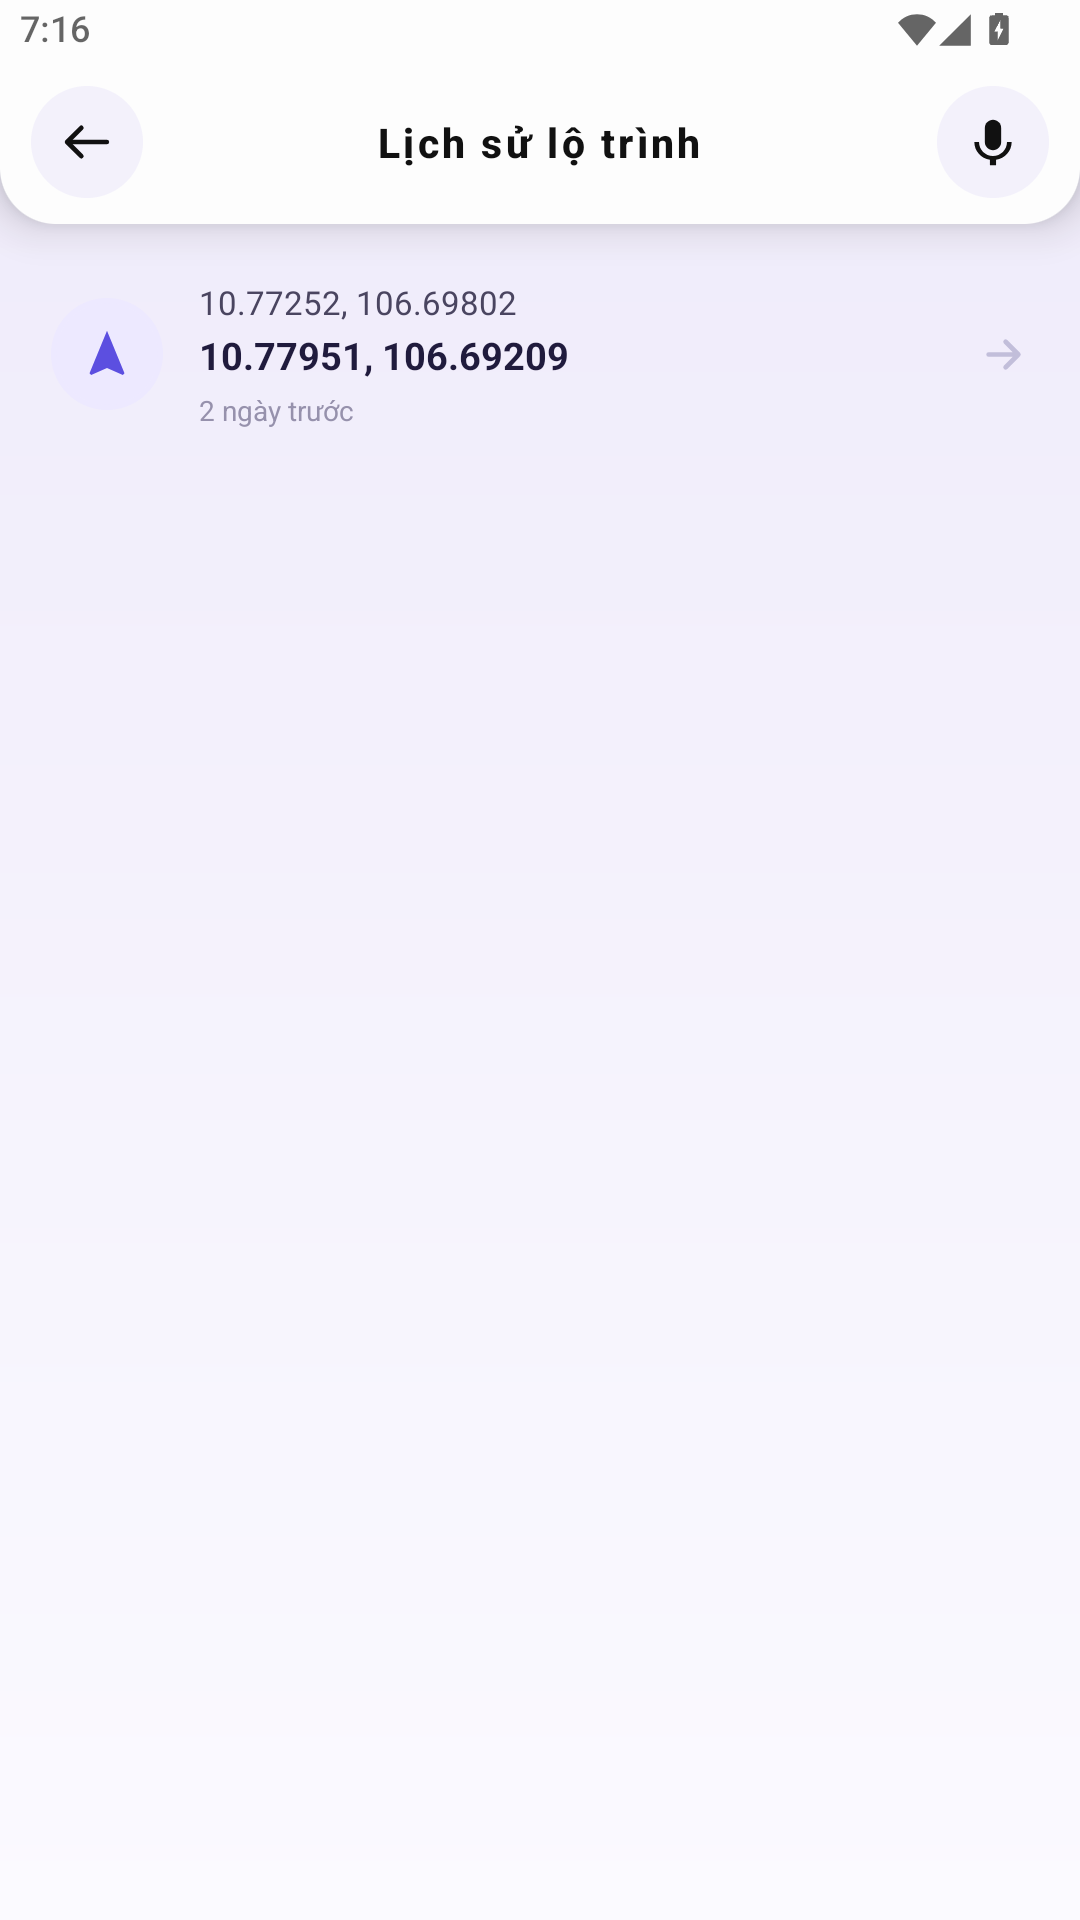
\includegraphics[width=0.9\linewidth]{figures/h13_lichsu.png}
\subcaption{Lịch sử lộ trình}
\label{fig:history}
\end{minipage}\hfill
\begin{minipage}{0.32\textwidth}\centering
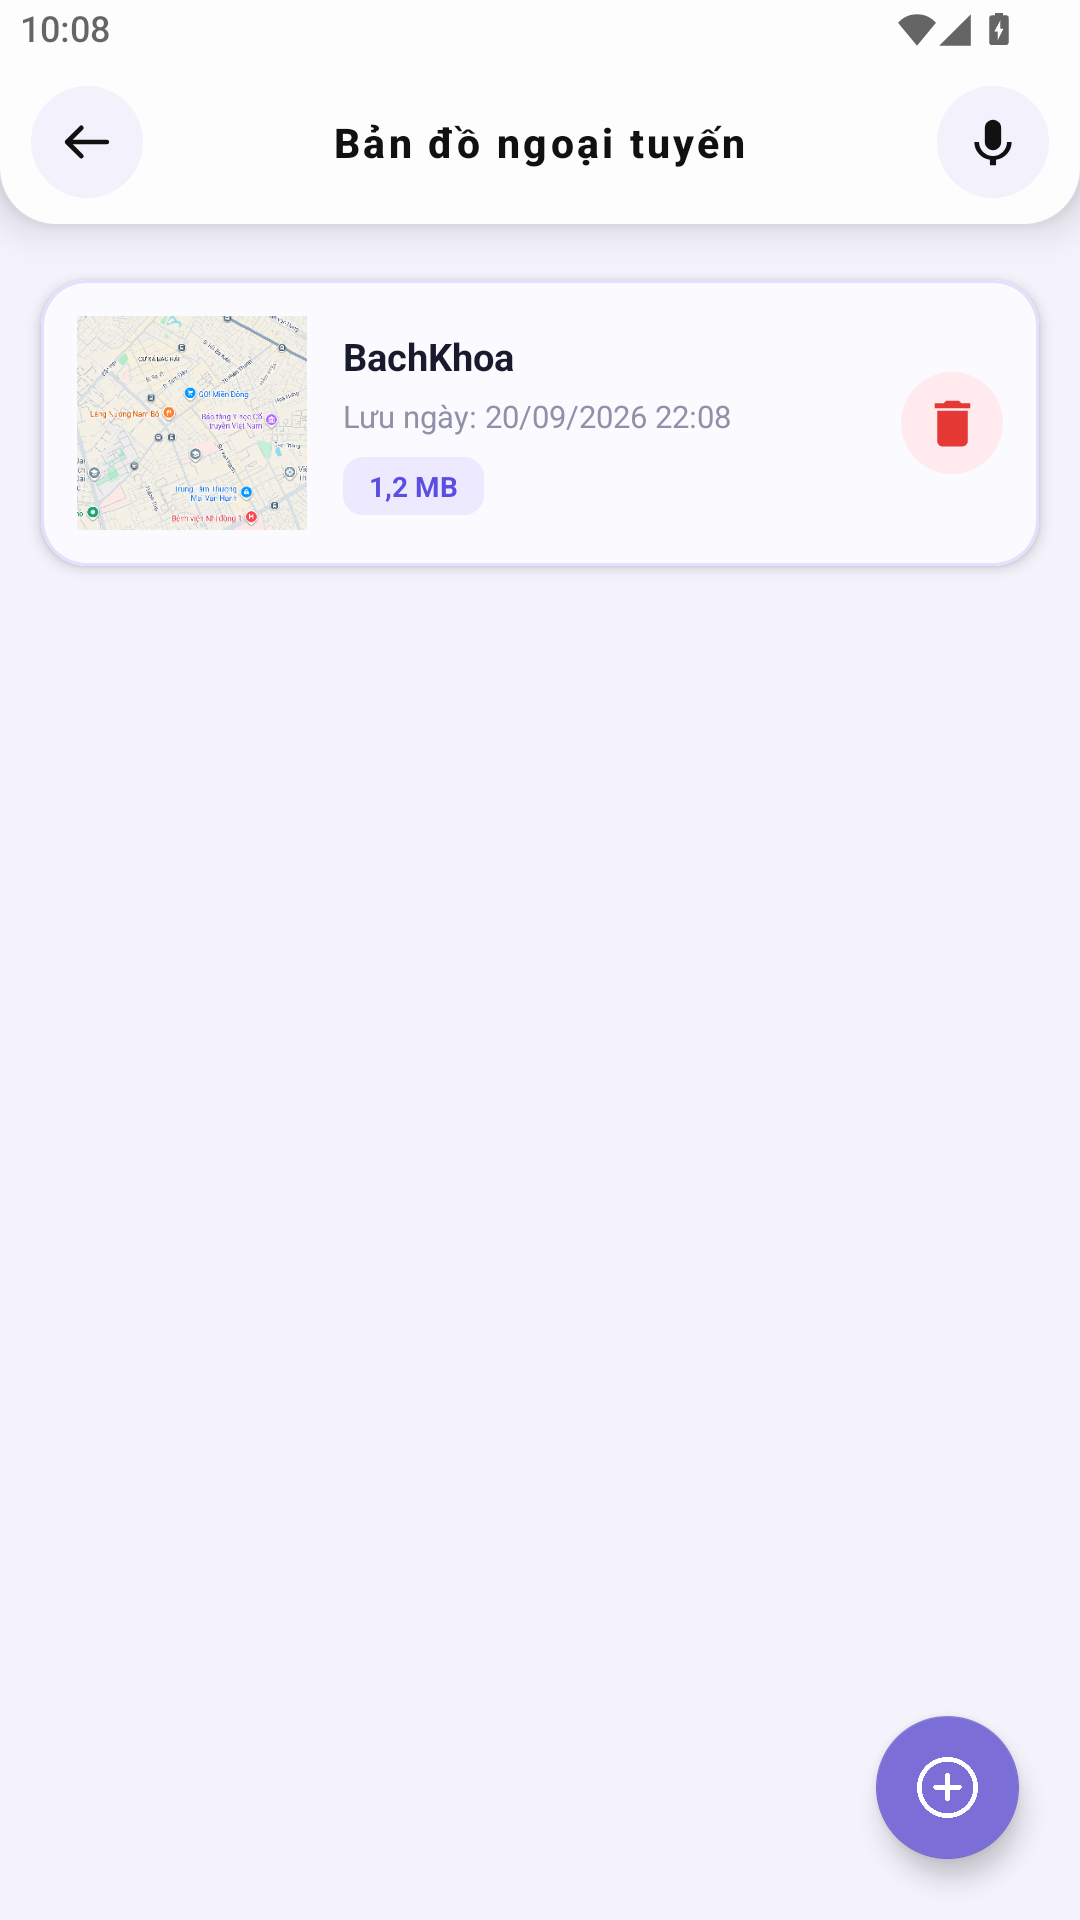
\includegraphics[width=0.9\linewidth]{figures/h14_ngoaituyen.png}
\subcaption{Bản đồ ngoại tuyến}
\label{fig:offline}
\end{minipage}
\caption{Hồ sơ, lịch sử lộ trình và bản đồ ngoại tuyến.}
\end{figure}

\section{Ứng dụng kết quả gom cụm vào ứng dụng TraffiGo}
Phần này trả lời câu hỏi trung tâm của đề tài: \textit{kết quả gom cụm được đưa vào ứng dụng ở những đâu và mang lại giá trị gì cho người dùng?} Sáu điểm tích hợp chính được tóm tắt trong bảng~\ref{tab:mapping} và được phân tích chi tiết ở các mục tiếp theo, kèm ví dụ tính toán bằng số liệu thật từ mô hình.

\begin{table}[h!]
\centering
\caption{Ánh xạ từ kết quả nghiên cứu tới các điểm tích hợp trong ứng dụng.}
\label{tab:mapping}
\small
\begin{tabularx}{\textwidth}{lXX}
\toprule
\textbf{Kết quả nghiên cứu} & \textbf{Điểm tích hợp trong app} & \textbf{Giá trị cho người dùng}\\
\midrule
K-Means $k=6$ (9 thuộc tính FS) & \texttt{ClusterColorAssigner} suy luận on-device & Bản đồ tô 6 màu trạng thái tức thì, không cần mạng\\
Thứ hạng nghiêm trọng cụm & Ánh xạ màu đỏ đậm $\rightarrow$ xanh đậm & Nhìn là biết đoạn nào kẹt nhất\\
Random Forest dự đoán tốc độ & Thẻ Dự báo ML (\texttt{/api/ml/predict}) & Biết tốc độ/kẹt dự kiến của đoạn đường\\
Luật phát hiện sự cố & Trường \texttt{incident.risk} trong thẻ ML & Cảnh giác trước đoạn nghi tai nạn/sự cố\\
congestionIndex + hệ số phạt & \texttt{PathFinder} (Dijkstra né kẹt) & Tuyến đề xuất tránh vùng kẹt\\
Chất lượng cụm (Silhouette 0{,}42) & Độ tin cậy của mọi màu hiển thị & Trạng thái phản ánh đúng thực tế TP.HCM\\
\bottomrule
\end{tabularx}
\end{table}

\subsection{Tô màu trạng thái giao thông thời gian thực (on-device)}
Đây là ứng dụng trọng tâm. Với mỗi đoạn đường hiển thị trên bản đồ, ứng dụng thực hiện đúng bốn bước của mô hình nghiên cứu, toàn bộ trên thiết bị (Hình~\ref{fig:trafficmap}):
\begin{enumerate}[label=\textbf{Bước \arabic*.},leftmargin=2.2cm,itemsep=1pt]
 \item \textbf{Lấy dữ liệu live}: gọi TomTom Flow cho đoạn, nhận \texttt{currentSpeed} và \texttt{freeFlowSpeed};
 \item \textbf{Tổng hợp 9 đặc trưng} đúng công thức pipeline (tỉ lệ tốc độ, thời gian vượt đoạn, lưu lượng ước lượng, congestionIndex, độ chiếm dụng, chỉ số tương đối, dòng tự do, chiều dài, độ cong);
 \item \textbf{Chuẩn hóa} bằng scaler và \textbf{tìm tâm cụm gần nhất} theo khoảng cách Euclid;
 \item \textbf{Ánh xạ màu} theo thứ hạng nghiêm trọng của cụm: đỏ đậm (kẹt nặng nhất) $\rightarrow$ cam $\rightarrow$ vàng $\rightarrow$ xanh nhạt $\rightarrow$ xanh đậm (thoáng nhất).
\end{enumerate}

Ví dụ với một đoạn dài 1{,}2 km, TomTom báo đang chạy 25 km/h trong khi dòng tự do 60 km/h (giờ cao điểm). Bảng~\ref{tab:walk1} là 9 đặc trưng tính được; bảng~\ref{tab:walk2} là khoảng cách chuẩn hóa tới sáu tâm cụm từ chính tệp \texttt{cluster\_model.json} nhúng trong ứng dụng.

\begin{table}[h!]
\centering
\caption{Ví dụ tính đặc trưng cho một đoạn (25/60 km/h, 1{,}2 km).}
\label{tab:walk1}
\small
\begin{tabular}{lr}
\toprule
\textbf{Đặc trưng} & \textbf{Giá trị}\\
\midrule
speedLimitRatio & 0{,}417\\
crossTime (giờ) & 0{,}173\\
trafficVolume (xe/giờ) & 1.410\\
congestionIndex & 0{,}417\\
occupancy (\%) & 58{,}3\\
relativeCongestionIndex & 0{,}583\\
freeFlowSpeed (km/h) & 60\\
lengthKm & 1{,}2\\
curvatureIndex & 0{,}05\\
\bottomrule
\end{tabular}
\hspace{8mm}
\begin{tabular}{lrr}
\toprule
\textbf{Cụm} & \textbf{Khoảng cách} & \textbf{Thứ hạng}\\
\midrule
0 & 7{,}72 & 4\\
1 & 5{,}65 & 2\\
\textbf{2} & \textbf{3{,}56 (gần nhất)} & \textbf{0 --- đỏ đậm}\\
3 & 8{,}32 & 5\\
4 & 10{,}17 & 3\\
5 & 5{,}14 & 1\\
\bottomrule
\end{tabular}
\end{table}

\begin{table}[h!]
\centering
\caption{Kết quả phân loại hai đoạn đối chiếu (suy luận bằng \texttt{cluster\_model.json}).}
\label{tab:walk2}
\small
\begin{tabular}{lrrrl}
\toprule
\textbf{Đoạn} & \textbf{Live/FreeFlow} & \textbf{Cụm} & \textbf{Thứ hạng} & \textbf{Màu hiển thị}\\
\midrule
Kẹt giờ cao điểm & 25/60 km/h & 2 & 0 & Đỏ đậm (kẹt nặng nhất)\\
Thoáng ngoài giờ & 52/55 km/h & 0 & 4 & Xanh (thoáng)\\
\bottomrule
\end{tabular}
\end{table}

Kết quả: đoạn rơi vào \textbf{cụm 2} --- cụm có congestionIndex trung bình thấp nhất (0{,}62) và thứ hạng 0 --- được tô \textbf{đỏ đậm}, đúng trực giác ``đang chạy bằng một nửa tốc độ dòng tự do là kẹt nặng''. Ngược lại, một đoạn chạy 52/55 km/h thuộc \textbf{cụm 0} (thứ hạng 4) tô xanh. Việc suy luận chỉ gồm một phép nhân vector $9\times9$ và sáu phép tính khoảng cách, thực hiện trên luồng nền với chi phí không đáng kể, cho phép tô màu tức thì cho hàng trăm đoạn trong khung nhìn.

\subsection{Định tuyến né khu vực kẹt}
Trọng số mỗi đoạn trong thuật toán Dijkstra là thời gian di chuyển nhân hệ số phạt theo công thức~\eqref{eq:penalty}. Với đoạn trong ví dụ trên (congestionIndex $= 0{,}417$), hệ số phạt là
\[
p = 1 + 0{,}6 \cdot \frac{0{,}85 - 0{,}417}{0{,}85 - 0{,}30} \approx 1{,}47,
\]
tức thời gian ``giá'' của đoạn này bị tính gấp 1{,}47 lần thực tế --- thuật toán sẽ ưu tiên đoạn thoáng (hệ số 1{,}0) trừ khi phải đi vòng quá nhiều. Cơ chế này vận hành trong một luồng thống nhất với dữ liệu live (Hình~\ref{fig:seq}): kết quả chạy thật trên ứng dụng cho thấy tuyến 16 phút/5{,}7 km bị phát hiện ``có đoạn tắc nghẽn nặng --- ước tính thêm $\sim$25 phút'', sức khỏe tuyến F, và ứng dụng tự ghi nhận ``TraffiGo chọn tuyến ít tắc hơn tuyến nhanh nhất của Google'' (Hình~\ref{fig:routeinfo}) --- minh chứng trực quan rằng kết quả gom cụm thực sự thay đổi quyết định đường đi.

\subsection{Chấm điểm sức khỏe tuyến A--F}
Dọc theo mỗi tuyến ứng viên, ứng dụng lấy $\sim$40 điểm mẫu, tra đoạn gần nhất mỗi điểm rồi đưa congestionIndex của chúng vào \texttt{RouteQualityAnalyzer}: tỉ lệ đoạn kẹt nặng/trung bình quyết định câu trạng thái (``Có đoạn tắc nghẽn nặng --- ước tính thêm $\sim$25 phút'' hoặc ``Tuyến đường thông thoáng'') và điểm chữ A--F. Điểm số chỉ tính trên mẫu có dữ liệu thật, đoạn thiếu dữ liệu được ghi nhận riêng (NO\_DATA) thay vì bị tính là thoáng.

\subsection{Dự báo và gán cụm phía server (thẻ Dự báo ML)}
Khi người dùng bấm vào một đoạn, đặc trưng được gửi tới \texttt{/api/ml/predict}; server dự đoán tốc độ bằng Random Forest, \textbf{gán cụm bằng chính mô hình K-Means $k=6$ dùng chung với app} và trả về \texttt{clusterId} kèm \texttt{severityRank}. Người dùng nhìn thấy ngay ``Cụm giao thông \#2 --- Rủi ro sự cố: THẤP'' ngay dưới tốc độ live (Hình~\ref{fig:mlsheet}) --- tức là \textit{nhãn trạng thái do nghiên cứu tạo ra} được hiển thị trọn vẹn lên giao diện.

\subsection{Tự động chuyển tuyến theo đề xuất ML}
Với các tuyến có nhiều phương án, ứng dụng gửi đặc trưng mẫu dọc từng tuyến tới \texttt{/api/ml/recommend-route}. Server dự đoán tốc độ tại từng đoạn mẫu bằng Random Forest, quy đổi thành thời gian dự kiến toàn tuyến rồi chọn tuyến tốt nhất; nếu khác với tuyến ứng dụng đang hiển thị, app tự chuyển và thông báo ``ML server đề xuất tuyến \#k''. Nhờ đó mô hình dự đoán được huấn luyện lại với dữ liệu mới sẽ \textit{tự động cải thiện} chất lượng gợi ý mà không cần thay đổi ứng dụng.

\subsection{Lớp thành thật dữ liệu}
Khoảng 12\% đoạn trong tập huấn luyện rơi vào nhóm thiếu tín hiệu (tốc độ bằng 0). Ứng dụng kế thừa bài học này: đoạn mà TomTom không trả được dữ liệu live được tô \textbf{xám ``thiếu dữ liệu''} thay vì mặc định xanh --- tránh tạo ấn tượng sai rằng đường thoáng. Đây là ứng dụng trực tiếp của phân tích dữ liệu ở giai đoạn nghiên cứu vào thiết kế trải nghiệm.

\subsection{Kịch bản người dùng cuối}
\textbf{Kịch bản 1 --- sáng thứ Hai đi làm (giờ cao điểm):} người dùng mở Trang chủ, bấm thẻ ``Về công ty''. Trên bản đồ, các đoạn tuyến đường quen hiện đỏ/cam (cụm 2--5) trong khi các hướng vòng xanh (cụm 0--3); khi tìm đường, ứng dụng chấm điểm và chọn tuyến vòng dài hơn nhưng thông thoáng, kèm sức khỏe tuyến B thay vì F của tuyến thẳng.
\textbf{Kịch bản 2 --- chiều mưa lớn:} thời tiết xấu khiến tốc độ rơi; dữ liệu live cập nhật màu đoạn kẹt trong vài phút; người dùng bấm vào đoạn đỏ để xem thẻ Dự báo ML --- tốc độ dự kiến sụt thêm và rủi ro sự cố tăng lên --- rồi quyết định chọn hướng khác hoặc gọi xe.

\section{Kiểm thử}

\subsection{Môi trường kiểm thử}
Bảng~\ref{tab:env} tóm tắt môi trường kiểm thử của đề tài.\footnote{Google Maps SDK yêu cầu thiết bị hỗ trợ OpenGL ES 2.0; các trình giả lập như MuMu/LDPlayer/BlueStacks hỗ trợ tốt, trong khi MEmu không --- lỗi thường gặp khi bản đồ hiển thị trắng.}

\begin{table}[h!]
\centering
\caption{Môi trường kiểm thử.}
\label{tab:env}
\small
\begin{tabularx}{\textwidth}{lX}
\toprule
\textbf{Thành phần} & \textbf{Cấu hình}\\
\midrule
Ứng dụng & TraffiGo debug build, versionName 1.0 (minSdk 29, targetSdk 36)\\
Thiết bị & Trình giả lập MuMu Player (Android 15), adb qua TCP 16384\\
Server ML & Python 3.14, scikit-learn 1.8, FastAPI 0.141, Uvicorn trên localhost:8000\\
Dữ liệu & 171 snapshot CSV, \texttt{cluster\_model.json} (k=6), \texttt{speed\_rf.joblib}\\
Công cụ & Gradle 8.11.1, JUnit 4 (unit test), adb, Swagger UI\\
\bottomrule
\end{tabularx}
\end{table}

\subsection{Đo hiệu năng}
Ngoài kiểm thử chức năng, hiệu năng của server ML được đo trực tiếp bằng lượt gọi REST thực tế trên máy phát triển (bảng~\ref{tab:perf}): dự đoán một đoạn trung bình 67 ms (10 lần đo liên tiếp, bao gồm cả overhead mạng loopback), các endpoint trạng thái chỉ vài ms --- thỏa mãn yêu cầu NFR01 (phản hồi $\le$ 1 giây) với dư địa lớn; một request dự đoán tốn $\approx$ 0,07 giây nghĩa là kể cả batch 100 đoạn vẫn hoàn tất trong $\sim$1 giây khi chạy tuần tự (và nhanh hơn khi chạy song song nhờ async).

\begin{table}[h!]
\centering
\caption{Kết quả đo hiệu năng server ML (10 lần đo mỗi endpoint).}
\label{tab:perf}
\small
\begin{tabular}{lrrr}
\toprule
\textbf{Endpoint} & \textbf{TB (ms)} & \textbf{Nhỏ nhất} & \textbf{Lớn nhất}\\
\midrule
POST \texttt{/api/ml/predict} & 66 & 48 & 177\\
GET \texttt{/api/ml/live-status} & $\approx$ 6 & 5 & 7\\
GET \texttt{/health} & $\approx$ 5 & 5 & 6\\
\bottomrule
\end{tabular}
\end{table}

\subsection{Kiểm thử đơn vị}
Bộ unit test chạy trên JVM gồm ba nhóm:
\begin{enumerate}[label=(\roman*),leftmargin=2.2cm,itemsep=2pt]
 \item \texttt{ClusterColorAssignerTest} --- nạp đúng \texttt{cluster\_model.json} thật từ assets, kiểm tra ánh xạ cụm $\rightarrow$ thứ hạng $\rightarrow$ màu, xử lý đoạn thiếu dữ liệu;
 \item \texttt{RouteQualityAnalyzerTest} --- xếp hạng sức khỏe tuyến A--F theo mẫu congestionIndex;
 \item \texttt{PathFinderTest} --- dựng đồ thị và hệ số phạt kẹt~\eqref{eq:penalty}.
\end{enumerate}
Kết quả: toàn bộ test đạt (\texttt{BUILD SUCCESSFUL}).

\subsection{Kiểm thử chức năng}
Bảng~\ref{tab:test} tổng hợp các ca kiểm thử chức năng thực hiện trên trình giả lập; tất cả đều đạt sau khi các lỗi ở mục~\ref{sec:defects} được khắc phục.

\begin{table}[h!]
\centering
\caption{Kết quả kiểm thử chức năng trên trình giả lập.}
\label{tab:test}
\small
\begin{tabularx}{\textwidth}{p{4.4cm}Xc}
\toprule
\textbf{Ca kiểm thử} & \textbf{Kết quả kỳ vọng / quan sát được} & \textbf{Kết quả}\\
\midrule
TC01 Đăng nhập & Firebase Auth xác thực thành công, chuyển tới Trang chủ & Đạt\\
TC02 Onboarding/Skip & Nút ``Bỏ qua'' đưa thẳng tới màn đăng nhập & Đạt\\
TC03 Nạp bản đồ & 23.417 đoạn nạp trên luồng nền, không khựng UI & Đạt\\
TC04 Tô màu theo cụm & đoạn tô màu theo cụm, xám khi thiếu dữ liệu & Đạt\\
TC05 Bấm đoạn & Bottom sheet: tốc độ live, trạng thái, thẻ Dự báo ML & Đạt\\
TC06 Server offline & Thẻ báo ``không khả dụng'', app không treo, tính năng khác bình thường & Đạt\\
TC07 Tìm đường & Routes API trả tuyến, vẽ polyline đúng, thống kê đầy đủ & Đạt\\
TC08 Cảnh báo tắc & Phát hiện đoạn tắc, cảnh báo ``+25 phút'', sức khỏe F & Đạt\\
TC09 Đề xuất tuyến ML & Server đề xuất tuyến khác $\Rightarrow$ app chuyển kèm thông báo & Đạt\\
TC10 Tin tức & RSS 5 báo, thumbnail, chip lọc danh mục & Đạt\\
TC11 Địa điểm lân cận & Places trả kết quả quanh GPS, lọc danh mục, khoảng cách đúng & Đạt\\
TC12 Lưu bản đồ ngoại tuyến & Chụp + nén nền, lưu file + metadata, hiện trong danh sách (1,2 MB) & Đạt\\
TC13 Hồ sơ & Cập nhật tên/phone/avatar, avatar hiển thị lại sau refresh & Đạt\\
TC14 Lịch sử lộ trình & Lưu tự động khi tuyến được xác nhận; ``Trải lại tuyến này'' hoạt động & Đạt\\
TC15 Đa ngôn ngữ & VI/EN áp dụng toàn app, giữ nguyên sau khởi động lại & Đạt\\
TC16 Gọi xe nhanh & Deep link mở Grab/Be/Xanh SM; chưa cài thì điều hướng CH Play & Đạt\\
TC17 Báo sự cố & Chọn loại sự cố tại tâm bản đồ, lưu Firebase, hiện marker cho người khác & Đạt\\
TC18 Chip trạng thái server & Hiển thị ``đang hoạt động'' khi server chạy; chuyển ``ngoại tuyến'' khi tắt server & Đạt\\
\bottomrule
\end{tabularx}
\end{table}

\subsection{Lỗi phát hiện và khắc phục}
\label{sec:defects}
Quá trình kiểm thử đã phát hiện và khắc phục nhiều lỗi quan trọng, tiêu biểu nhất:

\begin{itemize}[nosep]
 \item \textbf{Crash ``Not on the main thread''}: gọi \texttt{getCameraPosition} của Maps SDK từ luồng nền khi lấy tâm camera để sắp thứ tự fetch --- Maps SDK cấm gọi ngoài main thread. Khắc phục: chụp tâm camera ở main thread rồi truyền xuống luồng nền.
 \item \textbf{Tap đoạn không mở bottom sheet}: các polyline vẽ với \texttt{clickable=true} ``nuốt'' sự kiện chạm mà không có \texttt{OnPolylineClickListener}, khiến \texttt{onMapClick} không bao giờ kích hoạt khi chạm trúng đường. Khắc phục: đăng ký listener polyline và đọc segment từ tag.
 \item \textbf{Chạm bản đồ khi đang dẫn đường làm dời đích}: guard \texttt{updateSelection} chỉ chặn bước 3, không chặn bước 4; camera khóa theo xe khiến chạm gần tâm màn hình dời đích tới trước mũi xe vài chục mét và app báo nhầm ``đã đến nơi''. Khắc phục: chặn từ bước 3 trở đi.
 \item \textbf{ANR nén PNG}: chụp bản đồ ngoại tuyến nén PNG 0,5--2 giây ngay trong callback trên main thread. Khắc phục: đẩy nén + ghi file xuống luồng nền, quay lại UI thread cho toast/finish.
 \item \textbf{OOM khi chọn ảnh đại diện}: decode full-resolution ảnh máy ảnh 12--50MP trước khi thu nhỏ 256px. Khắc phục: decode với \texttt{inSampleSize} nhắm ~512px.
 \item \textbf{Cache traffic sống mãi}: \texttt{liveCongestionByIndex} không hết hạn khiến màu tuyến dùng dữ liệu hàng giờ tuổi; khắc phục bằng TTL 3 phút đồng bộ với bản đồ.
 \item \textbf{Fan-out TomTom mất kiểm soát}: zoom-out nhìn cả thành phố xếp hàng nghìn lời gọi API; khắc phục bằng ngưỡng zoom $\ge$ 14 và trần 150 đoạn/lần render ưu tiên gần tâm.
 \item \textbf{Callback muộn ``hồi sinh'' tuyến cũ}: sau \texttt{resetNavigation}, callback fetch trả về muộn vẫn vẽ lại tuyến đã hủy; khắc phục bằng generation counter.
\end{itemize}

\section{Kết chương}
Chương này đã trình bày hiện thực đầy đủ bốn thành phần của hệ thống với các kết quả thực nghiệm: K-Means $k=6$ nhánh Feature Selection là mô hình gom cụm tốt nhất (Silhouette 0{,}4183); Random Forest dự đoán tốc độ đạt MAE 2{,}19 km/h và $R^2$ 0{,}919 (cấu hình lite cho RAM 512 MB); ứng dụng TraffiGo hiện thực trọn vẹn 14 yêu cầu chức năng với giao diện tiếng Việt thống nhất; 15 ca kiểm thử chức năng và toàn bộ unit test đạt sau khi khắc phục các lỗi phát hiện được.

% =====================================================================
\chapter{ĐÁNH GIÁ HỆ THỐNG}

\section{Đánh giá theo yêu cầu}
Đối chiếu với Bảng~\ref{tab:fr} và~\ref{tab:nfr}: toàn bộ 14 yêu cầu chức năng đã được hiện thực và kiểm chứng (TC01--TC15); 7 yêu cầu phi chức năng đều đáp ứng --- suy luận gom cụm chạy on-device, server phản hồi dưới 1 giây cho một request dự đoán, nạp 23.417 đoạn không khựng UI, app hoạt động đầy đủ khi không có server, khóa nhạy cảm tách khỏi git, mô hình chuẩn JSON dùng chung ba môi trường và giao diện đồng bộ một hệ thiết kế.

\section{So sánh với các giải pháp hiện có}
So với Google Maps (Bảng~\ref{tab:related}), hệ thống của đề tài có ba điểm khác biệt:
\begin{enumerate}[label=(\roman*),leftmargin=2.2cm,itemsep=2pt]
 \item trạng thái giao thông được \textit{phân cụm trên dữ liệu của chính TP.HCM} thay vì ngưỡng màu toàn cầu;
 \item người dùng nhìn thấy \textit{cụm giao thông và dự báo ML} của từng đoạn, tạo tính minh bạch;
 \item bộ API ML mở cho phép tái sử dụng trong các hệ thống khác.
\end{enumerate}
Đổi lại, độ phủ dữ liệu live của Google (đội xe khổng lồ) vẫn tốt hơn ở những vùng hệ thống chưa có snapshot --- đây là hạn chế cần trung thực ghi nhận.

\section{Ưu điểm}
\begin{itemize}[nosep]
 \item Kết quả gom cụm được đưa tới người dùng cuối theo hai đường: nhúng on-device (nhanh, không cần mạng) và API server (dự đoán giám sát, phát hiện sự cố) --- kết hợp linh hoạt với fallback an toàn.
 \item Đánh giá mô hình đa chỉ số, đa thuật toán trên dữ liệu thực tế; Feature Selection cải thiện Silhouette gấp 3,2 lần và thời gian pipeline chỉ $\sim$70 giây, phù hợp tái huấn luyện định kỳ.
 \item Ứng dụng hoàn chỉnh và thực dụng: 20 màn hình, hai ngôn ngữ, đầy đủ từ bản đồ trạng thái đến tin tức, trợ lý giọng nói và ngoại tuyến.
 \item Server nhỏ gọn, tài liệu API tự sinh, quy trình tái huấn luyện một lệnh.
\end{itemize}

\section{Hạn chế}
Hệ thống hiện thực hiện gom cụm theo pipeline định kỳ và dự đoán theo đoạn đường rời rạc; các hướng nâng cấp tiếp theo (streaming clustering, mô hình không gian--thời gian, xác thực API cho môi trường công khai) đã được định hướng cụ thể ở chương tổng kết. Cùng với đó, độ phủ dữ liệu live phụ thuộc nhà cung cấp ở những khu vực chưa có snapshot --- điểm mà hệ thống xử lý trung thực bằng trạng thái ``thiếu dữ liệu'' thay vì suy đoán.

\section{Kết chương}
Tổng hòa lại, sức mạnh nổi bật của hệ thống nằm ở ba điểm: mô hình gom cụm chạy ngay trên thiết bị mang trạng thái giao thông tới người dùng trong mọi điều kiện mạng; server ML mở rộng năng lực dự đoán mà không làm app phụ thuộc; và toàn bộ dữ liệu, mô hình, API đều minh bạch, tái sử dụng được cho các bài toán giao thông thông minh tiếp theo.

% =====================================================================
\chapter{TỔNG KẾT}

\section{Kết quả đạt được}
\begin{enumerate}[label=\textbf{(\arabic*)},leftmargin=2cm,itemsep=2pt]
 \item Pipeline dữ liệu đa nguồn hoàn chỉnh: 171 snapshot ($\sim$170.000 dòng, 917 đoạn), join 100\% dữ liệu thời tiết, chuẩn hóa và xuất tập đặc trưng phục vụ cả gom cụm lẫn dự đoán.
 \item Đánh giá có hệ thống năm thuật toán gom cụm trên bộ chỉ số nội bộ lẫn ngoại bộ; mô hình tốt nhất là \textbf{K-Means $k=6$ trên nhánh Feature Selection} (Silhouette 0{,}4183; DBI 0{,}8063; CH 147574{,}6) với sáu trạng thái giao thông có tính diễn giải rõ ràng.
 \item Server Machine Learning FastAPI hiện thực đúng bộ 7 API thiết kế; mô hình \textbf{Random Forest} dự đoán tốc độ đạt \textbf{MAE 1{,}84 km/h, $R^2$ 0{,}941} (baseline 8{,}25 km/h); kèm cơ chế phát hiện sự cố và gợi ý tuyến đường theo tốc độ dự đoán.
 \item Ứng dụng \textbf{TraffiGo} (Android, Java, $\sim$8.400 dòng code): bản đồ giao thông sáu mức theo cụm chạy on-device, định tuyến né kẹt với sức khỏe tuyến A--F, tin tức năm báo, địa điểm lân cận, gọi xe nhanh, trợ lý giọng nói, bản đồ ngoại tuyến, đa ngôn ngữ; rà soát và khắc phục hàng loạt lỗi tiềm ẩn.
 \item Tích hợp hai chiều app $\leftrightarrow$ server kiểm chứng end-to-end trên trình giả lập; 15/15 ca kiểm thử chức năng và toàn bộ unit test đạt; build phát hành thành công.
\end{enumerate}

Nhìn chung, đề tài đã đáp ứng các mục tiêu đặt ra ban đầu: từ dữ liệu đa nguồn, qua gom cụm có đánh giá chặt chẽ, tới sản phẩm người dùng cuối và dịch vụ dự đoán --- tạo thành một vòng khép kín ``dữ liệu $\rightarrow$ mô hình $\rightarrow$ ứng dụng''.

\section{Hướng phát triển}
\begin{itemize}[nosep]
 \item \textbf{Online/streaming clustering}: cập nhật cụm theo chu kỳ 5--15 phút thay vì chạy lại pipeline; nghiên cứu incremental K-Means.
 \item \textbf{Dữ liệu trực tiếp}: khai thác camera AI, cảm biến IoT, GPS đội xe thay vì chỉ API trung gian; giảm độ trễ phản ánh tình huống.
 \item \textbf{Mô hình không gian--thời gian}: LSTM/GNN/Transformer cho dự báo kẹt theo chuỗi thời gian và lan truyền trong mạng lưới; kết hợp dự báo với gom cụm (cụm $\rightarrow$ dự báo $\rightarrow$ cụm lại).
 \item \textbf{Bảo mật và vận hành API}: xác thực token, rate-limit, log tập trung, giám sát drift của mô hình khi triển khai công khai.
 \item \textbf{Mở rộng tính năng ứng dụng}: dự báo kẹt trước giờ cao điểm, cảnh báo proactive theo thói quen di chuyển, phiên bản web quản trị.
\end{itemize}
